% Editorial consolidation 2026-10-11
% Self-contained manuscript; empirical values are generated from archived runs.
\documentclass[12pt]{article}
\usepackage[margin=0.75in]{geometry}
\usepackage[T1]{fontenc}
\usepackage{amsmath,amssymb,amsthm,booktabs,array}
\usepackage[hidelinks]{hyperref}
\usepackage{xurl}
\usepackage{microtype}
\usepackage{placeins}
\usepackage{pgfplots}
\pgfplotsset{compat=1.18}
\renewcommand{\topfraction}{0.95}
\renewcommand{\bottomfraction}{0.9}
\renewcommand{\textfraction}{0.05}
\renewcommand{\floatpagefraction}{0.75}
\setlength{\emergencystretch}{1em}
\newtheorem{proposition}{Proposition}
\newtheorem{corollary}{Corollary}
\newcommand{\F}{\mathcal{F}}
\newcommand{\R}{\mathbb{R}}
\newcommand{\M}{\mathcal{M}}
\newcommand{\Oset}{\mathcal{O}}
\newcommand{\clip}{\operatorname{clip}}
\title{Auditing Machine-Learning Forecasts with Aggregate Targets: Exact Deterministic and Randomized Recovery}
\author{Jishan Kapoor\\
Independent Researcher\\
Toronto M4Y 1C9, Canada\\
Corresponding author: \href{mailto:kapoorjishan19@gmail.com}{kapoorjishan19@gmail.com}}
\date{}
\begin{document}
\maketitle

\begin{abstract}
Missing verification targets can make machine-learning model comparisons
depend on imputation assumptions. We study fixed-record squared-error audits
when nonnegative targets and disjoint aggregate measurements constrain the
missing values. Paired-loss cancellation gives sharp comparison intervals.
Sorted windows and dynamic programming solve deterministic budgeted recovery,
and deterministic adaptation cannot improve its minimax width. We then
derive an exact randomized batch method: a weighted-endpoint pricing oracle
and a compact flow formulation replace enumeration of query subsets. For one
block with $m$ unknown coordinates, $r\geq2$ retained coordinates, and positive optima, the
deterministic-to-randomized worst-expected-width ratio is at most $m/r$;
separated clusters attain the bound when $r$ divides $m$. Every realized
comparison interval remains valid. The energy evaluation contains 34 meter
series and 3,729 test days, with a frozen replication on 30 additional
consumers and 3,210 days. All permitted direct forecast-archive copies are
incorporated before the historical audit. On the original public Portugal
panel, randomization reduces normalized worst expected width by 9.88\%
relative to exact deterministic recovery, but increases observed expected
width by 17.45\%. A separate public rainfall application establishes two
strict daily comparisons from nine naturally accumulated records; one
survives a declared aggregate-tolerance sensitivity. Secondary optimization
and the additional-consumer analysis preserve the observed tradeoff;
independent checks reproduce the calculations. The contribution is an exact tractable recovery method and a
sharp limit on the value of randomization, with explicit separation between
robust guarantees, realized performance, and unmeasured retrieval costs.
\end{abstract}
\noindent\textbf{Keywords:} machine learning; model evaluation; robust optimization;
randomized recovery; partial identification; aggregate observations.

\section{Introduction}
Evaluating a fixed machine-learning forecast requires verification targets
as well as saved predictions. When targets are missing, deletion changes
the evaluated record and imputation makes its score depend on a chosen
completion. Production monitoring systems explicitly join predictions to
subsequently collected actuals \cite{azuremonitor,awsmonitor}. The question
here is which model comparisons follow from the available measurements
alone, and which additional targets would most reduce the remaining ambiguity.
The audit operates on saved predictions; it requires neither model gradients
nor an additional fitted missing-shape model.

Aggregate observations provide useful constraints without specifying that
shape. Differences between cumulative meter readings constrain the energy
within their interval \cite{canada}. NorPEN documents missing high-frequency
transmissions alongside more reliably collected hourly billing registers
\cite{norpen}. Elexon's procedures reconcile interval sums with register
advances and recover a missing interval from the advance and the other
readings \cite{elexon}; AEMO provides for replacing substituted readings
when actual data are recovered \cite{aemo}. These sources motivate retained
totals and subsequent correction. They do not establish that exact totals
survive every outage, or that selectively retrieving individual readings
is cheaper than retrieving an entire gap.

We represent the unknown targets by a common feasible set of nonnegative
values consistent with the observed readings and disjoint aggregate totals.
A strict forecast ordering is established only if every feasible completion
gives that ordering. For squared error, the unknown squared target cancels
from the paired loss difference, leaving a linear objective. Sharp extrema
then depend on the residual energy and the range of forecast disagreement
within each block. Thus a large missing fraction can still permit a decision,
while a small gap can remain consequential.

The main contribution is an exact recovery method for this structured
evaluation problem. Its three results distinguish established optimization
tools from the specialized reductions developed here:
\begin{enumerate}
\item Deterministic worst-width recovery reduces to sorted retained windows
and budget allocation across blocks. A zero-answer argument shows that
deterministic adaptation cannot improve this minimax value.
\item Randomized recovery admits an exact weighted-endpoint pricing oracle
and a compact budget-flow linear program. The solution generates executable
batches satisfying a hard reading budget without enumerating all query
subsets. The hidden record is fixed before the random draw.
\item For one block with $m$ missing and $r\geq2$ retained coordinates and positive optima,
the deterministic-to-randomized worst-expected-width ratio is at most $m/r$.
Separated clusters attain this bound when $r$ divides $m$.
\end{enumerate}
The deterministic extension to independently bounded totals and a secondary
minimax-regret option are retained in the appendices. The randomized theory
uses exact totals; neither recovery objective maximizes empirical certification.

The experiments test both the applicability and the limits of these results.
In the energy audit, permitted direct copies from the saved forecast archive
reconstruct most masked targets before recovery, leaving a small incremental
certification benefit from exact rather than greedy allocation. Randomization
improves its robust objective but worsens observed expected width; this
tradeoff persists under target-independent secondary optimization and on
additional consumers. Naturally accumulated precipitation records provide
a separate zero-query application: some comparisons follow from surviving
totals even though individual forecast scores are not identified.

The practical output is therefore a defensible comparison interval and an
exactly optimized recovery policy for a stated uncertainty criterion.
The evidence does not establish general ranking-accuracy superiority over
imputation or measured retrieval savings. The following sections define the
observation model, derive deterministic recovery, and develop the randomized
method in Section~\ref{sec:randomized-recovery}. The results lead with the
archive-consistent audit; the appendices preserve the restricted-record
experiments and supporting designs.

\section{Related Work and Contribution Boundary}
Partial identification formalizes what can be learned without selecting a
single completion of missing information \cite{manski}. Maia Polo et al.
apply this perspective to performance evaluation and model selection under
weak supervision \cite{polo}. Bessac and Naveau study forecast scoring with
imperfect observations using a probabilistic observation model \cite{bessac}.
Botacin and Gomes examine delayed labels and resource constraints in
realistic malware-model evaluation \cite{botacin2025}. Delayed-target
monitoring itself is therefore established context; the present method
addresses sharp finite-record comparisons and minimax-width recovery under
aggregate target constraints.
The abstract of the 2026 road-safety preprint by Elbasri and Elamrani Abou
Elassad (SSRN, \url{https://doi.org/10.2139/ssrn.7176879}) describes
conditional score and model-difference envelopes under changing spatial
units; this literature comparison is limited to its public abstract.
Thus incomplete-outcome evaluation and model-difference
envelopes are established concepts.

Patton \cite{patton} characterizes losses whose expected forecast rankings
are preserved under conditionally unbiased volatility proxies. His loss
representation includes a target-only term that cancels in pairwise
comparisons, leaving affine target dependence. Our squared-loss cancellation
is an instance of this established structure. We instead bound a fixed
historical comparison over every nonnegative completion compatible with
retained energy measurements, then use that feasible set to plan recovery.

Energy-constrained reconstruction also predates this work. Copy-Paste
Imputation (CPI) preserves the total energy of gaps while borrowing shapes
from related observations \cite{cpi}. Hu et al. develop constrained Monte
Carlo disaggregation and uncertainty estimation \cite{hu}. Schaffer et al.
use cumulative information when preparing a large heat-meter dataset
\cite{heat}. These methods aim to construct or sample plausible high-resolution
trajectories. A sampled set of plausible trajectories need not contain the
extrema needed to establish a comparison over \emph{all} measurement-compatible
trajectories.

Our objective is the paired forecast-error difference, rather than the
reconstruction error of an imputed load profile. We retain all completions
allowed by the stated measurements and report exactly which finite-record
comparisons survive that ambiguity. The direct paired calculation is also
compared with separately bounded individual errors, so the empirical benefit
of respecting the shared unknown target can be assessed.

Appendix~\ref{app:regret} applies the standard minimax-regret criterion
\cite{savage,manskiregret} to these bounds as a secondary decision option.
We do not claim to introduce partial identification, minimax regret, linear
optimization, conservation constraints, or a forecasting architecture. The
specific contribution is their specialization to retained meter totals,
including sharp formulas, a useful identifiability diagnostic, an exact
budgeted batch-recovery rule, and evidence about the resulting audit decisions.

Active evaluation already studies which labels to acquire for assessing
fixed predictors. Sawade et al.\ \cite{sawade} directly address paired model
comparison, including squared-loss regression, by choosing an importance
sampling distribution to improve asymptotic test power. Hara et al.\
\cite{hara} develop adaptive acquisition aimed at reducing the variance of
estimated test-loss differences. These works establish budgeted acquisition
for model comparison; our contribution concerns a different objective:
the worst remaining range of a fixed-record loss difference under retained
energy constraints.

Related active testing and worst-case sensor selection address model
evaluation and measurement choice more broadly \cite{active,sensorsel}.
Costly observation within robust optimization is also established.
Vayanos et al.\ \cite{ddid} formulate decision-dependent information
discovery and develop tractable approximations for multistage problems.
Our recovery rule specializes this general setting to a scalar contrast
over nonnegative interval values with disjoint exact sums. This structure
permits an exact sorted-window calculation and budget-allocation dynamic
program.

The retained-coefficient subproblem is a one-dimensional minimum-diameter
subset problem, within the classical family studied by Aggarwal et al.
\cite{aggarwal}. Neither this sorting subproblem nor dynamic programming
is claimed as new. The specialized result is the reduction of worst-case
comparison uncertainty after record recovery to this tractable structure,
its exact allocation across retained-total blocks, and its deterministic
adaptivity characterization under the stated information model.


Chen et al.~\cite{chen2026} study robust selection after querying uncertain
parameters under budgeted uncertainty. Their subsequent item-selection
problem differs from reducing a fixed contrast's range over continuous
aggregate-constrained targets. Iancu and Trichakis~\cite{iancu2014} address
dominated robust optima; our secondary policy audit applies this established
principle rather than claiming it as a new concept.
Table~\ref{tab:closest-work} distinguishes the nearest settings. Exactness
refers to each work's own stated problem, not a common benchmark or a claim
that one method dominates the others.
\begin{table}[htbp]\centering\footnotesize
\caption{Closest methodological settings and the contribution boundary.}
\label{tab:closest-work}
\begin{tabular}{>{\raggedright\arraybackslash}p{0.16\linewidth}>{\raggedright\arraybackslash}p{0.25\linewidth}>{\raggedright\arraybackslash}p{0.25\linewidth}>{\raggedright\arraybackslash}p{0.23\linewidth}}\toprule
Work & Information and uncertainty & Acquisition and objective & Solution or guarantee\\\midrule
Maia Polo et al.~\cite{polo} & Weak labels and partially identified performance & No coordinate-recovery design; classification metric bounds & Convex optimization under its observation assumptions\\
Hara et al.~\cite{hara} & Unlabeled test pool and surrogate label model & Adaptive labeling; variance of estimated test-loss differences & Unbiased estimation with a surrogate-based acquisition approximation\\
Chen et al.~\cite{chen2026} & Queried parameters and budgeted uncertainty & Queries followed by item selection; robust objective or feasibility & General hardness, special-case algorithms and mixed-integer formulations\\
Kawase and Sumita~\cite{kawase2024} & Set family and objective scenarios & Randomized feasible-set choice; worst expected objective & General oracle/separation framework and approximation results\\
This work & Nonnegative targets with disjoint exact sums & Fixed-pair recovery; deterministic width or randomized expected width & Exact window/DP and compact LP; deterministic adaptivity identity and sharp one-block gap\\
\bottomrule\end{tabular}\end{table}

\section{Observation Model and Evaluation Target}

Table~\ref{tab:notation} collects the main symbols. The development first
defines the common feasible record and sharp comparison bounds, then treats
deterministic batch recovery. The randomized method in
Section~\ref{sec:randomized-recovery} also assumes exact totals; it minimizes
worst expected width when the hidden record is fixed before the batch draw.
The deterministic extension to interval totals is given separately in
Appendix~\ref{app:interval-theory}.

\begin{table}[htbp]\centering\small
\caption{Main notation. Quantities refer to one fixed model pair and its
declared evaluation record; exact and interval totals are distinguished.}
\label{tab:notation}
\begin{tabular}{p{0.23\linewidth}p{0.70\linewidth}}\toprule
Symbol & Meaning\\\midrule
$N$, $y_i$, $a_i$, $b_i$ & Target count, target value, and two fixed predictions.\\
$\Oset$, $\M$ & Observed coordinates (including permitted reconstructions) and remaining missing coordinates.\\
$I_g$, $\M_g$, $m_g$ & Disjoint aggregate block, its missing coordinates, and their count.\\
$\F$ & All target records compatible with the declared observations and aggregate constraints.\\
$E_g$; $[\ell_g,u_g]$ & Exact residual total; residual-total interval after subtracting observed values.\\
$D(y)$, $c_i$ & Paired MSE difference $L_a(y)-L_b(y)$ and coefficient $2(b_i-a_i)/N$ of a missing target.\\
$B$, $Q$, $S_g(Q)$ & Hard reading budget, queried batch, and unqueried coordinates in block $g$.\\
$W(Q,y)$ & Remaining comparison-interval width after querying $Q$ on record $y$.\\
$\pi$, $R_B$ & Distribution over admissible batches and its optimal worst expected width.\\
$m$, $r$, $D_B$ & In the one-block gap theorem: missing count, retained count $r=m-B$, and optimal deterministic worst-case width.\\
\bottomrule\end{tabular}
\end{table}


\subsection{Fixed forecasts and a common record}
Let $p^{(j)}\in\R^N$ be the predictions of candidate $j$ for the same $N$
scheduled nonnegative targets. For the energy experiments, predictions are
issued before these targets occur and are frozen before evaluation masks
are imposed. The separate precipitation application uses documented
retrospective reforecasts and naturally accumulated observations. The
finite-record mean squared error (MSE) is
\begin{equation}
 L_j(y)=\frac{1}{N}\sum_{i=1}^N(p_i^{(j)}-y_i)^2.
 \label{eq:loss}
\end{equation}
All candidates use identical targets and the same denominator. The primary
unit is kWh per interval, so the loss is in kWh$^2$. Equal-weight root mean
squared error (RMSE) has
the same ordering as MSE on this common record, although its numerical
difference is not the MSE difference bounded below.

We condition on a declared evaluator-access regime and treat forecast
vectors as fixed. The original daily \emph{restricted-record} regime supplies
the current evaluation record's predictions, observed targets and totals;
it does not supply later forecast records or retained feature caches.
Any target reconstructed from additional authorized records must first be
added to the observed set. Section~\ref{sec:archive-access} evaluates this
augmentation using all available saved test persistence forecasts.
Sharpness and recovery optimality below are relative to the resulting
information set, not every record held anywhere in a forecasting system.

The observed coordinates $\Oset$ have fixed recorded values $o_i$.
The remaining coordinates $\M$ are unavailable to the evaluator.
Disjoint register blocks $I_g$ have retained total-energy constraints
$T_g^-\leq\sum_{i\in I_g}y_i\leq T_g^+$. The total may include both
observed and missing coordinates. In the primary model,
\begin{equation}
 \F=\left\{y:\begin{array}{l}
 y_i=o_i\ (i\in\Oset),\quad y_i\geq0\ (i\in\M),\\
 T_g^-\leq\sum_{i\in I_g}y_i\leq T_g^+\quad\forall g
 \end{array}\right\}.
 \label{eq:feasible}
\end{equation}
Every missing coordinate belongs to exactly one block with a finite upper
total. Nonnegativity and these totals make $\F$ bounded. This default needs
no maximum load estimated from the training data and imposes no smoothness
assumption on a missing load shape.

\subsection{Counter semantics and feasibility}
For missing indices $\M_g=I_g\cap\M$, subtract the surviving interval
energies before optimization:
\begin{align}
 r_g^-&=T_g^- -\sum_{i\in I_g\cap\Oset}o_i,\\
 r_g^+&=T_g^+ -\sum_{i\in I_g\cap\Oset}o_i,\\
 \ell_g&=\max(0,r_g^-),\qquad u_g=r_g^+.
 \label{eq:residual}
\end{align}
If $\ell_g>u_g$, the information is inconsistent and the method returns a
data-quality failure. A block with no missing values must likewise have its
known sum inside its supplied total interval. These are exact-arithmetic
feasibility conditions. The reference API rejects infeasibility; the
experimental pipeline's roundoff convention is specified below and is
distinct from uncertainty in a physical measurement.

An exact total is defensible for differences of retained readings of the
same monotone cumulative counter when the targets are the intervening
counter increments. This is a statement about the recorded counter scale,
not about an error-free measurement of physical energy. Integrating a few
instantaneous power samples does not in general produce exactly the same
quantity. Counter resets, rollover, unit mismatches, import/export mixing,
and timestamp mismatch must be checked before applying the constraints.
The primary experiments use nonnegative consumption. Signed net exchange
requires an appropriate signed feasible set and cannot automatically inherit
the nonnegative formulas.

Where the retained total has a defensible uncertainty range, its interval
is applied before subtracting observed values. If the observed interval
values themselves are uncertain, treating them as exact is inappropriate;
their uncertainty must also be included in $\F$. The 1\% and 5\% ranges
used below are controlled sensitivity settings, not estimated meter-error
distributions or claimed metrological specifications.

\section{Sharp Comparisons and Decision Guarantees}
\subsection{Cancellation of the unknown quadratic term}
For two fixed forecasts $a,b$, put $D(y)=L_a(y)-L_b(y)$. Expanding gives
\begin{align}
 D(y)&=K+\sum_{i\in\M}c_i y_i,\label{eq:linear}\\
 c_i&=\frac{2(b_i-a_i)}{N},\\
 K&=\frac{\sum_{i=1}^N(a_i^2-b_i^2)
       +2\sum_{i\in\Oset}(b_i-a_i)o_i}{N}.
\end{align}
The $y_i^2$ terms cancel because both forecasts are evaluated against the
same unknown truth. All observed contributions and all scheduled targets
remain in the calculation.

\begin{proposition}[Sharp bounds from exact totals]
Suppose $\F$ is nonempty and each nonempty missing block has an exact
residual total $E_g\geq0$. Then the attainable range of $D$ is exactly
$[D^-,D^+]$, where
\begin{align}
 D^-&=K+\sum_g E_g\min_{i\in\M_g}c_i,\label{eq:sharpmin}\\
 D^+&=K+\sum_g E_g\max_{i\in\M_g}c_i.
 \label{eq:sharp}
\end{align}
Blocks with no missing coordinates contribute zero to these sums.
\end{proposition}
\begin{proof}
For $E_g>0$, $\sum_i c_i y_i/E_g$ is a convex combination of the
coefficients in block $g$. Its minimum and maximum are attained by placing
the whole residual energy on an index with the smallest or largest
coefficient. For $E_g=0$, nonnegativity forces every missing value to zero.
Disjoint blocks permit simultaneous attainment of these extrema. Convexity
of $\F$ and linearity of $D$ imply attainment of every intermediate value.
\end{proof}

Thus $D^+<0$ establishes that $a$ has smaller MSE for every admissible
completion, while $D^->0$ establishes that $b$ does. Otherwise a strict
ordering does not follow from these constraints. If $D^-<0<D^+$,
the two extremal completions explicitly demonstrate opposite orderings.
An interval touching zero may establish a weak ordering but does not
establish a strict winner. The implementation conservatively labels such
cases unresolved.

In exact arithmetic, sharpness also establishes completeness of this
strict-decision rule.
If $0\in[D^-,D^+]$, the feasible set contains a tie, so no rule whose
strict winner must be valid for every member of the same feasible set can
certify a strict winner. If the interval straddles zero, opposite winners
are feasible as well. Thus stronger guaranteed decisions require additional
information or additional assumptions, rather than a different treatment
of the same unconstrained missing shape. The recovery method below adds
information by retrieving selected values.

\subsection{Why some gaps are informative and others are not}
\begin{corollary}[Width and identified contrasts]
For exact residual totals,
\begin{equation}
 D^+-D^- = \frac{2}{N}\sum_g E_g
 \left[\max_{i\in\M_g}(b_i-a_i)
       -\min_{i\in\M_g}(b_i-a_i)\right].
 \label{eq:width}
\end{equation}
For a positive-energy block, its contribution vanishes precisely when
the forecast contrast is constant across its missing coordinates.
\end{corollary}
The corollary follows by subtracting the two sharp bounds. It explains why
an audit cannot be characterized by its missing fraction alone. A constant
bias adjustment can be evaluated from the aggregate even if all intervals
within that block are absent. A shape-changing adjustment may remain
unresolved. A block with only one missing value is reconstructed exactly
by its total. In the two-target scenarios, fine aggregate blocks can
therefore reconstruct the missing truth. The six- and twelve-target
conditions also test multiple missing coordinates within a retained block;
resolution in these conditions is important when assessing usefulness
beyond single-value reconstruction.

More generally, for the missing-target set
$\F_{\M}=\{x\geq0:Ax=e\}$, any coefficient vector
$c=A^\top\lambda$ gives a fixed contrast $c^\top x=\lambda^\top e$.
The necessary and sufficient condition is that $c$ is orthogonal to
$\operatorname{span}(\F_{\M}-\F_{\M})$. Equivalence to membership in the row space
of $A$ requires that feasible variations span its null space, as occurs
when a strictly positive feasible point exists. A zero-energy block can
fix coordinates and must not be used to claim the unqualified converse.

Refining a retained total into compatible sub-block totals or recovering
additional true readings shrinks $\F$, so sharp comparison intervals cannot
widen. This is a direct consequence of optimizing over nested sets.

\subsection{Uncertain totals and optional physical limits}
For a nonempty missing block with residual sum in $[\ell_g,u_g]$, let
$c_g^{\min}$ and $c_g^{\max}$ denote the minimum and maximum coefficient.
Its exact contributions become
\begin{align}
 d_g^-&=\min(\ell_g c_g^{\min},u_g c_g^{\min}),\\
 d_g^+&=\max(\ell_g c_g^{\max},u_g c_g^{\max}).
 \label{eq:tolerance}
\end{align}
These replace the block terms in \eqref{eq:sharpmin} and \eqref{eq:sharp}. The coefficient scan
and scalar endpoint choice remain linear in the number of missing values.

Documented coordinate bounds $l_i\leq y_i\leq h_i$ can tighten the result.
For this extension, initialize at $l$, sort coefficients increasingly, and
allocate the mandatory residual energy to the smallest coefficients subject
to capacity. Allocate any optional energy only where the coefficient is
negative. Negating the coefficients gives the maximum. The cost is
$O(m_g\log m_g)$ per block. With bounded coordinates and an uncertain total,
the optimum can use an interior total; evaluating just two fixed-total
solutions is not a valid general replacement for this procedure.
Overlapping aggregate constraints require a general linear program instead
of independent block allocation. The primary study uses no capacity bounds.

Fixed nonnegative loss weights satisfying $\sum_i w_i>0$ are accommodated by replacing $1/N$ with
$w_i/\sum_k w_k$ in each summand. If the target is average power with
unequal interval durations $d_i$, transform $x_i=d_i y_i$ in the energy
constraint; the linear objective coefficient for $x_i$ is then
$2w_i(b_i-a_i)/(d_i\sum_k w_k)$. Merely sorting the unadjusted coefficients
would solve a different problem. Our experiments forecast interval energy
directly.

\subsection{Why separate error bounds can be weaker}
Let $l_a,u_a$ and $l_b,u_b$ be sharp individual loss bounds on the same
$\F$. Independent subtraction gives $[l_a-u_b,u_a-l_b]$, which contains
the direct paired interval. It may combine two extremal completions that
cannot simultaneously be the truth.

For example, take $a=(1,1)$, $b=(2,2)$, and unknown nonnegative
$y_1+y_2=2$. The individual MSE ranges are $[0,1]$ and $[1,2]$, giving
an independent difference interval $[-2,0]$. The paired difference is
exactly $-1$, so the direct method establishes the strict ordering.
Conversely, with $a=(0,2)$ and $b=(2,0)$ under the same total, the
paired difference spans $[-4,4]$; no strict winner can be justified.
These are analytical examples, not experimental measurements.

For completeness, the individual squared-error minimum over a nonnegative
simplex is obtained by Euclidean projection of the prediction vector onto
that simplex. The maximum is attained at a vertex. For exact residual
energy $E$ and missing prediction vector $p$,
\begin{align}
 s^-&=\|p-\Pi_{\Delta(E)}(p)\|_2^2,\\
 s^+&=\sum_i p_i^2+E^2-2E\min_i p_i,
 \label{eq:separate}
\end{align}
where $\Delta(E)=\{x\geq0:\sum_i x_i=E\}$. These standard calculations
provide the same-information comparator in the experiments. For uncertain
totals the minimizing total is
$\clip(\sum_i\max(p_i,0),\ell,u)$; the maximum is the larger endpoint
value of the convex quadratic in \eqref{eq:separate}.

\section{Budgeted Recovery of Missing Readings}
A comparison that remains unresolved can guide data repair.
Suppose an operator can retrieve at most $B$ missing interval-energy values
from a meter buffer or a secondary archive. Each recovered target has unit
cost. The policy chooses one batch before seeing any of the requested
values. The budget represents a limit on records retrieved and validated;
equal record cost is an explicit abstraction, not a measured staffing or
communication cost. The budget counts recovered targets, not network packets or
cumulative-register endpoint requests. This extension applies when such
retrieval is operationally possible; it does not recover permanently lost
information without an additional measurement source. The budget and
optimality statement apply to one specified model pair. Different pairs
can request different values; a joint recovery plan for all candidates
would require a different multi-objective optimization.

\subsection{An exact objective before reading recovery}
For an exact-total block let $Q_g\subset\M_g$ be the queried indices and
$S_g=\M_g\setminus Q_g$ the remaining missing indices. If $S_g$ is nonempty,
the comparison-width contribution after observing the query answers is
\begin{equation}
 W_g(Q_g,y)=\left(E_g-\sum_{i\in Q_g}y_i\right)
 \left(\max_{i\in S_g}c_i-\min_{i\in S_g}c_i\right).
 \label{eq:querywidth}
\end{equation}
The constant term of the comparison changes too, but does not affect its
width. The worst possible width over the currently feasible targets is
\begin{equation}
 H_g(Q_g)=E_g\left(\max_{i\in S_g}c_i-\min_{i\in S_g}c_i\right),
 \label{eq:worstquery}
\end{equation}
because the queried values can all be zero while the remaining coordinates
carry the full residual energy. A singleton $S_g$ has zero range. Thus the
last missing target need not be queried: its exact total already determines
it after the other missing values are recovered. Zero-energy blocks also
need no recovery.

\begin{proposition}[Optimal batch recovery within a block]
Sort the $m_g$ missing-target coefficients as
$c_{g,(1)}\leq\cdots\leq c_{g,(m_g)}$. For $0\leq k\leq m_g-1$, the
smallest worst-case width obtainable by recovering $k$ values is
\begin{equation}
 h_g(k)=E_g\min_{1\leq s\leq k+1}
 \{c_{g,(s+m_g-k-1)}-c_{g,(s)}\}.
 \label{eq:window}
\end{equation}
An attaining batch queries the coordinates outside a minimizing consecutive
window of $m_g-k$ sorted coefficients.
\end{proposition}
\begin{proof}
Equation~\eqref{eq:worstquery} reduces the problem to retaining $m_g-k$
coefficients with minimum range. Any such subset spans at least $m_g-k$
ordered entries. A consecutive window of that size within its span has no
larger range. Conversely each consecutive window is a feasible retained
subset. Minimizing over the $k+1$ possible windows proves the formula;
the zero-query-energy completion attains its worst-case width.
\end{proof}

\subsection{Allocation across retained-total blocks}
Disjoint blocks permit simultaneous attainment of their worst cases.
For allocation, index only blocks with $m_g\geq2$ and $E_g>0$ by
$g=1,\ldots,G$; all other blocks have zero width and require no query.
Consequently the global problem is
\begin{equation}
 \min_{\substack{k_g\in\{0,\ldots,m_g-1\}\\\sum_g k_g\leq B}}
 \sum_g h_g(k_g),
 \label{eq:allocation}
\end{equation}
with empty and already determined blocks assigned zero cost and no queries.
Dynamic programming gives an exact solution. If $V(g,b)$ is the minimum
cost for the first $g$ blocks using exactly $b$ recoveries, then
\begin{equation}
 V(g,b)=\min_{0\leq k\leq\min(b,m_g-1)}
 \{V(g-1,b-k)+h_g(k)\}.
\end{equation}
Initialize $V(0,0)=0$, other states to infinity, and select the smallest
$V(G,b)$ over $b\leq B$. Store the minimizing window and allocation to
return actual interval indices. Coefficient ties and equal-cost allocations
use deterministic index-based rules. The algorithm uses only archived
forecasts, surviving values, and retained totals before requesting the batch.

An implementation has four steps: remove determined blocks; sort each
remaining block's coefficients while retaining their interval indices;
enumerate the minimum-range window at every feasible local budget and
apply the allocation recurrence; then recover the selected indices and
map them to record timestamps. Put $q=\min(B,\sum_g(m_g-1))$ and
$K_g=\min(q,m_g-1)$. Sorting costs
$O(\sum_g m_g\log m_g)$; enumerating the scalar window costs requires
$O(\sum_g(K_g+1)^2)$ operations. The allocation recurrence has at most
$O(G(q+1)^2)$ transitions. A backpointer implementation needs $O(q+1)$
rolling scalar states and $O(G(q+1))$ backpointer storage, in addition to
the sorted inputs and local window choices. The released readable Python
prototype instead copies and sorts query-index tuples at each transition,
adding up to $O(q\log(q+1))$ work per transition and $O((q+1)^2)$
auxiliary tuple storage. The reported timings include this bookkeeping;
they do not describe a backpointer-only implementation.

\begin{proposition}[A limitation of one-step greedy recovery]
For the greedy batch rule that repeatedly chooses the coordinate giving
the largest immediate decrease in worst-case width, no positive universal
approximation factor for width reduction holds, even with one block and
two queries. The ratio of its remaining width to the optimal remaining
width is unbounded, including instances with a strictly positive optimum.
\end{proposition}
\begin{proof}
Take one block of residual energy $E=3$, budget two, and coefficients
$(0,\varepsilon/2,\varepsilon,1,1)$, where $0<\varepsilon<1/2$.
Greedy uniquely removes the first coefficient and then the second,
leaving worst-case width $3(1-\varepsilon)$. The minimum-range
three-element window is $(0,\varepsilon/2,\varepsilon)$, so the exact
rule removes the two unit coefficients and leaves width $3\varepsilon$.
The ratio of width reductions is
$\varepsilon/(1-\varepsilon)\to0$, whereas the ratio of remaining
widths is $(1-\varepsilon)/\varepsilon\to\infty$.
\end{proof}
These coefficients are realized by nonnegative five-target forecasts
$a_i=0$ and $b_i=5c_i/2$. Their initial comparison interval contains
zero: its endpoints are $K=-5/2-25\varepsilon^2/16$ and $K+3$.
Independent enumeration of every subset of at most two queries verifies
the executable examples. This is an analytical limitation of the width
heuristic; it does not assert frequent greedy failure or an approximation
claim for empirical certification rates.

For an analytical example, a block with $E=6$ and coefficients
$(0,1,2,10)$ initially has width 60. One query at the coefficient 10
guarantees remaining width at most 12, regardless of the answer returned.
This illustrates the objective; it is not a measured
experiment or an assertion that typical loads have this shape.

The optimality statement concerns \emph{worst-case interval width} for
nonadaptive batches, exact totals, nonnegative uncapped targets, and equal
query costs. It does not optimize realized width, the probability of
certification, or the number of correct empirical decisions. An alternative
batch can perform better at the realized load profile. Optimizing average behavior under a stochastic load model would require
an explicitly specified target distribution.
Section~\ref{sec:interval-recovery} gives a separate batch extension for
independently bounded totals. Unequal query costs and capacity constraints
remain outside the implemented recovery rules.
Optimal batches for different budgets need not be nested. Their optimal
worst-case widths cannot increase with budget, but their realized widths
or resolution rates need not be monotone across independently chosen batches.

\subsection{Deterministic adaptivity cannot improve this minimax width}
Adaptive and fixed information have a substantial optimal-recovery
literature \cite{osipenko}. Classical sufficient conditions involving
central symmetry do not directly apply to a positive-energy simplex with
more than two coordinates. The proof below instead uses a feasible
zero-answer transcript for the restricted coordinate-query geometry.
The following statement uses the specific
nonnegative exact-sum geometry and a hard query budget.
\begin{corollary}[Deterministic adaptive recovery]
Under the assumptions above, let $W^*(B)$ be the optimal value in
\eqref{eq:allocation}. Among all deterministic policies that select each
next query using the answers already observed and request at most $B$
values for every feasible record, the smallest worst-case terminal
comparison width is exactly $W^*(B)$.
\end{corollary}
\begin{proof}
A query whose answer is already determined---a zero-residual block or its
last missing coordinate---can be omitted and its answer simulated in the
policy's history. This preserves its terminal information while using no
more queries. For the resulting nonredundant policy, answer zero to each
query. The transcript is feasible: each positive-energy block retains at
least one unqueried coordinate, to which its remaining energy can be
assigned at termination. Let $Q_0$ be the queried set on this transcript.
Its terminal width is $\sum_g E_g\operatorname{range}(c_{\M_g\setminus Q_0})$,
which is at least $W^*(B)$ because $|Q_0|\leq B$. A completion assigning
the residual energies to unqueried coordinates realizes this transcript.
Every deterministic adaptive policy consequently has worst-case width
at least $W^*(B)$. The optimal fixed batch is itself a deterministic policy,
giving the reverse inequality.
\end{proof}
This deterministic result does not rule out gains in average width or
empirical resolution. Section~\ref{sec:randomized-recovery} characterizes
the separate randomized worst-expected-width objective.


\subsection{Extension to independently bounded totals}
The deterministic batch objective also admits an exact extension when each
disjoint aggregate lies in a specified interval. Appendix~\ref{app:interval-theory}
gives the optimizer and proof; the randomized theory below concerns exact
totals only.

\section{Randomized Recovery under a Hard Budget}
\label{sec:randomized-recovery}

Randomization permits a different guarantee from deterministic minimax
recovery. We retain exact disjoint totals, nonnegative uncapped targets,
unit query costs, and one fixed forecast contrast. The benchmark first incorporates permitted direct persistence copies
and aggregate-determined values. Sharpness is relative to the declared
feasible set; inverse constraints from other fitted predictors are not
included in the evaluated archive regime.
Remove zero-energy, singleton, and constant-coefficient blocks, whose width
is already zero. Index the remaining blocks by $g=1,\ldots,G$.
If none remain, the optimal width is zero and no query is needed.
Let $\mathcal Q_B$ contain batches with at most $B$ queries in total and
at most $m_g-1$ in block $g$; querying its final coordinate is redundant.
A policy selects $Q\sim\pi$ before reading its answers. The hidden record
$y\in\F$ is fixed before this random draw: the adverse completion may
depend on $\pi$, but cannot depend on the realized batch.

\subsection{Expected width and an exact finite linear program}
Write $S_g(Q)=\M_g\setminus Q$, let $d_g(S)$ denote the coefficient range
on $S$, and set $d_g(S)=0$ for a singleton or empty set. Define
$v_{gi}(Q)=\boldsymbol{1}\{i\in S_g(Q)\}d_g(S_g(Q))$.
Equation~\eqref{eq:querywidth} gives
\begin{equation}
 W(Q,y)=\sum_g\sum_{i\in\M_g}y_i v_{gi}(Q),\qquad
 R_B=\min_{\pi\in\Delta(\mathcal Q_B)}\sup_{y\in\F}
       \mathbb E_{Q\sim\pi}W(Q,y).
 \label{eq:random-objective}
\end{equation}
Here $\Delta(\mathcal Q_B)$ is the set of distributions over admissible
batches. The budget holds for every draw, rather than only in expectation.
The coefficients $c_i$ already include the MSE normalization in
\eqref{eq:linear}.

\begin{proposition}[Finite characterization]
\label{prop:random-finite}
For every batch distribution,
\begin{equation}
 \sup_{y\in\F}\mathbb E_\pi W(Q,y)
 =\sum_g E_g\max_{i\in\M_g}\mathbb E_\pi v_{gi}(Q).
 \label{eq:random-value}
\end{equation}
Consequently $R_B$ is the value of the primal and dual programs
\begin{equation}
 \begin{aligned}
 \min_{\pi,t}\quad &\sum_g E_g t_g,\\
 \text{subject to}\quad
 &\sum_Q\pi_Qv_{gi}(Q)\leq t_g\quad(g,i),\qquad
   \sum_Q\pi_Q=1,\quad\pi_Q\geq0;
 \end{aligned}
 \label{eq:random-primal}
\end{equation}
\begin{equation}
 \begin{aligned}
 \max_{w,\eta}\quad &\eta,\\
 \text{subject to}\quad
 &\eta\leq\sum_g\sum_i w_{gi}v_{gi}(Q)\quad(Q\in\mathcal Q_B),\\
 &\sum_i w_{gi}=E_g,\quad w_{gi}\geq0.
 \end{aligned}
 \label{eq:random-dual}
\end{equation}
The variables $t_g$ and $\eta$ are free; the primal inequalities imply
$t_g\geq0$.
\end{proposition}
\begin{proof}
Interchanging finite sums makes the expected width linear in each
block's target vector. Its maximum over a nonnegative simplex of mass
$E_g$ places that mass on a largest expected coefficient. The blocks are
independent, proving \eqref{eq:random-value}. Introducing their maxima
gives the primal. Linear-programming duality gives the stated dual;
the primal is feasible and has a finite optimum.
\end{proof}

Mixed-strategy robust optimization and dual separation are established
methods. Kawase and Sumita provide a general framework based on weighted
scenario optimization \cite{kawase2024}; Mastin, Jaillet, and Chin study
randomized minmax regret and improvements over deterministic strategies
\cite{mastin2015}. The specialization here is the conditional-width
geometry, the exact coordinate-recovery oracle and compact formulation
below, and the sharp comparison with deterministic adaptive recovery.

\subsection{An exact pricing oracle}
To separate \eqref{eq:random-dual}, minimize
$\sum_{g,i}w_{gi}v_{gi}(Q)$ over admissible batches. Within a block, order
coefficients increasingly, breaking ties by original coordinate index.
For local budget $k$, put $r=m_g-k$. If $r\geq2$, fix the first and last
retained positions $l<u$, with $u-l+1\geq r$. The least cost for these
endpoints is
\begin{equation}
 (c_{g,(u)}-c_{g,(l)})
 \left(w_{g,(l)}+w_{g,(u)}+
       \sum_{i\in T_{g,l,u,r}}w_{g,(i)}\right),
 \label{eq:random-pricing}
\end{equation}
where $T_{g,l,u,r}$ contains the $r-2$ smallest interior weights.
Every retained subset has such endpoints; once they are fixed, its range
is fixed and these interior choices minimize its nonnegative weighted
cost. Enumerate the endpoints, assign cost zero when $r=1$, and apply
the budget-allocation recurrence across blocks. This supplies exact
polynomial-time separation for rational input. Unlike deterministic
minimum-range recovery, an optimal weighted retained set need not be
a consecutive coefficient window.

\subsection{A compact program and an executable batch distribution}
The following formulation avoids a variable for every possible batch.
Set $q=\min(B,\sum_g(m_g-1))$. Any smaller batch can be padded to $q$
queries without widening its conditional interval for any record, so
requiring exactly $q$ loses no optimality for this objective.
The case $B=0$ is obtained directly from the original width formula.

Construct a directed acyclic graph with nodes $(g,b)$ for completed
blocks $0\leq g\leq G$ and budgets $0\leq b\leq q$. For each admissible
$k$ and endpoint pair $(l,u)$ of a retained set of size $r=m_g-k\geq2$,
create an edge $e=(g,b,k,l,u)$ from $(g-1,b)$ to $(g,b+k)$.
For $r=1$, use a single canonical zero-width edge. Impose nonnegative
unit flow $p_e$ from $(0,0)$ to $(G,q)$, with conservation at all other
nodes. Impossible nodes and edges may be omitted.

For an endpoint edge, introduce interior joint inclusion masses satisfying
\begin{equation}
 0\leq z_{ei}\leq p_e\quad(l<i<u),\qquad
 \sum_{l<i<u}z_{ei}=(r-2)p_e.
 \label{eq:random-hypersimplex}
\end{equation}
Its endpoint inclusion masses are $p_e$; interior inclusion masses are
$z_{ei}$, and all others are zero. Denote these by $\alpha_{ei}$ and
put $d_e=c_{g,(u)}-c_{g,(l)}$. Zero-width edges contribute zero.
The compact program minimizes $\sum_gE_gt_g$ subject to the flow
constraints, \eqref{eq:random-hypersimplex}, and
\begin{equation}
 \sum_{e\text{ for block }g}d_e\alpha_{ei}\leq t_g
 \quad(g,i).
 \label{eq:random-compact}
\end{equation}

\begin{proposition}[Exact compact representation]
\label{prop:random-compact}
This program has value $R_B$ and yields an attaining distribution with
at most $B$ queries in every batch. For $B\geq1$, a safe unpruned bound
on its numbers of variables and constraints is
$O(B\sum_g\min(B,m_g)m_g^3)$.
For one block with a fixed local budget, only $O(m_g^3)$ variables are needed.
\end{proposition}
\begin{proof}
A distribution over batches induces flows along their budget paths and
the corresponding endpoint and interior inclusion masses, satisfying
all constraints. Conversely, a nonnegative unit flow on an acyclic graph
decomposes into source-to-sink paths. For any edge with $p_e>0$,
the vector $(z_{ei}/p_e)_{l<i<u}$ belongs to
$\{x\in[0,1]^{u-l-1}:\sum_i x_i=r-2\}$. This hypersimplex is the convex
hull of the indicators of its $(r-2)$-element subsets. To see integrality,
any nonintegral feasible vector has at least two fractional entries;
opposite small perturbations of those entries express it as the midpoint
of two distinct feasible vectors, so it is not a vertex.
Thus each positive-flow edge admits a distribution of legal interiors.
Sample a flow path and, conditionally on each selected edge, such an
interior subset. Every resulting batch uses exactly $q$ queries and
has the coordinate coefficients in \eqref{eq:random-compact}. Hence
the two formulations attain the same objective. There are $O(B)$ budget
layers per block, $O(\min(B,m_g))$ local budget choices, $O(m_g^2)$
endpoint choices, and $O(m_g)$ interior variables per endpoint edge,
giving the bound.
\end{proof}

The decomposition is constructive: sample outgoing edges proportionally
to their flows and sample a fixed-cardinality subset with the conditional
interior marginals. For the latter, cumulative marginal intervals and a
uniform offset in $[0,1)$ give systematic sampling with the required
cardinality and marginal probabilities. Preserve the original coordinate
indices when returning the queried complements. The implementation reports
floating-point feasibility and marginal repairs; its numerical solution
is not an outward-rounded proof certificate.

\subsection{A sharp separation from deterministic adaptive recovery}
\begin{proposition}[One-block randomization gap]
\label{prop:random-gap}
For one exact-total block with $E>0$, $m$ missing coordinates, and
$0\leq B\leq m-2$, put $r=m-B$ and
$h=\min_{|S|=r}d(S)$. Let $D_B=Eh$ be its optimal deterministic
worst-case width, which also equals the optimum over deterministic
adaptive policies. Then
\begin{equation}
 \frac{r}{m}D_B\leq R_B\leq D_B.
 \label{eq:random-gap}
\end{equation}
When $r$ divides $m$, the lower bound is attained by instances with
$D_B>0$, so the factor $m/r$ cannot be improved in general.
\end{proposition}
\begin{proof}
Pad every batch to $B$ queries. Each retains $r$ coordinates, and therefore
\[
 \sum_{i=1}^m\mathbb E_\pi v_i(Q)
 =r\mathbb E_\pi d(S(Q))\geq rh.
\]
Its largest expected coordinate coefficient is at least $rh/m$;
\eqref{eq:random-value} proves the lower bound. A point mass at the
deterministic optimal batch proves the upper bound. Equality of
deterministic batch and adaptive optima follows from the preceding
zero-answer argument.

For sharpness, form $m/r$ coefficient clusters, each containing $r$
equally spaced points of range $h>0$, and separate adjacent clusters
by gaps strictly greater than $h$. Every $r$-point subset has range
at least $h$, and a complete cluster attains it. Uniformly retain one
cluster and query its complement. Each coordinate then has expected
coefficient $hr/m$, giving $R_B=Ehr/m$.
\end{proof}

If $D_B=0$, both optima are zero and their ratio is undefined.
The separation concerns randomized nonadaptive batches versus all
deterministic adaptive policies; it does not establish optimality among
randomized adaptive policies. Every realized sharp comparison interval
contains the comparison value for the fixed record and for every completion
consistent with its query answers. The improvement is in worst expected width, not a bound
on every realized width, a higher certification probability, or measured
retrieval savings. The result does not extend here to overlapping or
uncertain totals, physical caps, or heterogeneous query costs.


\subsection{Choosing among equally robust policies}\label{sec:tie-selection}
The primary minimax objective need not select a unique policy. Robust
optima can be dominated away from their worst case, a general issue studied
by Iancu and Trichakis~\cite{iancu2014}. For example, take one block with
$E=1$, $c=(0,2,4,12)$ and $B=2$. A policy retaining pairs
$\{1,2\},\{1,3\},\{2,3\}$ with probabilities $0.4,0.2,0.4$ has expected
coefficient vector $(1.6,1.6,1.6,0)$. Retaining $\{1,2\}$ and $\{3,4\}$
with probabilities $0.8,0.2$ instead gives $(1.6,1.6,1.6,1.6)$.
Both have optimal worst expected width $1.6$: dual weights
$(0.2,0.6,0.2,0)$ certify this value. The first policy is never worse,
and is strictly better when $y_4>0$.

Write $e_{gi}(\pi)=\mathbb E_\pi v_{gi}(Q)$. After finding $R_B$, a
target-independent secondary rule minimizes
\begin{equation}
 H(\pi)=\sum_g\frac{E_g}{m_g}\sum_{i\in\M_g} e_{gi}(\pi)
 \quad\text{subject to}\quad
 \sum_g E_g\max_i e_{gi}(\pi)\leq R_B.
 \label{eq:secondary-policy}
\end{equation}
This is expected width at the uniform-within-block feasible completion,
not an estimated load distribution. It is a linear objective on the
optimal face of the finite LP. A policy that is no worse at every feasible
record and strictly better somewhere would also improve $H$, contradicting
secondary optimality. Thus this standard refinement removes dominated
expected-width functions; it need not identify a unique distribution or
maximize certification.

We also check the stronger requirement of never worsening the archived
policy $\pi_0$. Expected-width dominance is equivalent to
$\sum_g E_g\max_i[e_{gi}(\pi)-e_{gi}(\pi_0)]\leq0$.
Block epigraph variables, free in sign, encode this condition linearly.
Minimizing $H$ over that set preserves a primary-optimal $\pi_0$'s robust
value in exact arithmetic. The two refinements answer different questions:
the first chooses a reference criterion on the optimal face; the second
only allows improvements over the particular saved policy. Neither uses
hidden targets or guarantees that certification improves.

\subsection{Interpreting the robust objective}
A four-coordinate family displays the full tradeoff without selecting a
favorable observed record. Let $c=(0,\delta,L,L+\delta)$, $L\geq2\delta>0$,
and $B=2$. An optimal deterministic policy retains the first pair; its width
is $E\delta\lambda$, where $\lambda$ is that pair's share of total energy.
Equally mixing the two within-cluster retained pairs gives width
$E\delta/2$ in expectation at every feasible record and attains the lower
bound in Proposition~\ref{prop:random-gap}. It improves on that deterministic
policy when $\lambda>1/2$, ties at $1/2$, and worsens when $\lambda<1/2$.
The robust guarantee protects against an unspecified feasible allocation
chosen before the random draw; it is not an average-load or decision-cost
optimum. More generally Proposition~\ref{prop:random-gap} implies
$(D_B-R_B)/D_B\leq B/m$ for positive one-block optima. The low-budget
$(m,B)=(60,4)$ and $(120,6)$ fixtures therefore permit at most $6.67\%$
and $5\%$ relative robust gains, motivating the larger budget fractions in
the computational study below.

\section{Experimental Design}
\subsection{Data sources and chronological splits}
The primary evaluation uses 34 consumption series from three public sources
(Table~\ref{tab:data}). The Portugal panel uses the first 30 eligible meter
IDs in the ordered UCI ElectricityLoadDiagrams20112014 file \cite{portugal}.
Eligibility requires at least 99\% finite and more than 95\% positive
training-hour values. The training year is 2013; test windows are the first
28 days of January, April, July, and October 2014. The original end-stamped
15-minute average-kW readings are shifted to interval starts and converted
to hourly energy by summing four values and dividing by four.

The UCI French household trace \cite{uci} supplies a separate scale and
load pattern. Training uses 2008--2009 and testing uses eligible days in
2010. Hourly kWh is the sum of 60 minute-average kW values divided by 60;
all 60 readings must be valid. For both UCI sources, the spring and autumn
clock-transition dates and target days whose 1-, 2-, or 7-day lags touch
them are excluded in training and testing. This prevents documented local
time-grid artifacts from contaminating the features. Every eligible day
must contain all 24 targets and all required causal features. The retained
totals in these two sources are constructed from the complete trace before
masking; they are not separate backup-register measurements.

The third source contains actual cumulative Discovergy consumption counters
released with the BLEM study \cite{blem}. We use the first three consumer
IDs in the pinned source version identified in the supplement. Each raw
series contains 175,201 readings on an uninterrupted three-minute grid,
without counter decreases. Hourly energy is calculated from integer
counter differences at exact UTC hour endpoints, using the source's
$10^{-10}$ conversion to kWh. Training uses January--September 2017 and
testing uses October--December 2017, subject to complete-day and feature
availability. First and last partial days are excluded. Here the retained
six-hour or daily totals can be obtained directly from the recorded
counter endpoints. Removing interval targets is still an artificial outage:
the experiment assumes these endpoints remain available and does not
measure an independent communication channel's survival rate.

\begin{table}[t]
\centering\normalsize
\caption{Data retained after feature and quality filters. Training and
test counts are days per series; totals are test meter-days.}
\label{tab:data}
\begin{tabular}{lrrrr}
\toprule
Source & Meters & Train & Test & Total\\
\midrule
Portugal & 30 & 357 & 107 & 3,210\\
French household & 1 & 587 & 246 & 246\\
Counter meters & 3 & 266 & 91 & 273\\
\bottomrule
\end{tabular}
\end{table}

The study contains 3,729 test meter-days. A dated local protocol records
the design and amendments for counter data, daylight-saving handling,
information-flow checks, and whole-period comparisons. This is not a
registered study. The household trace was used during implementation
development and is reported separately. After inspecting an earlier
four-model analysis, we replaced weekly persistence with an MLP in a
dated expansion of the candidate model set. An initial neural run exposed training-iteration-limit
warnings; a documented amendment increased the training allowance based
on those training diagnostics, retaining the architecture and all other
hyperparameters. The final configuration was checked for training convergence
before the final evaluation run. The retained split therefore is not a new blind
validation panel. No hyperparameters were selected using the revised
evaluation outcomes. All reported empirical values come from the revised
run; the earlier results are not mixed with it. The underlying records
remain historical (2010--2017), rather than newly collected 2026 loads.


\subsection{Forecasts and information cutoffs}
The four candidates are previous-day persistence, ridge regression,
histogram gradient boosting, and a multilayer perceptron (MLP) neural
network. Boosting and the MLP provide nonlinear AI models; persistence and
ridge provide simple references. Each forecast supplies all 24 targets at
the start of a day. In this retrospective benchmark, issue time is a
simulated historical day-start cutoff enforced through feature timestamps;
these are not contemporaneously logged vendor forecasts.
Features for target hour $h$ are lagged values at 24, 48, and 168 hours,
the mean of the previous day, and sine/cosine encodings of hour, weekday,
and month. All features are available at the common issue time. The
regression models share parameters across the 24 target hours.

Ridge uses training-only standardization and regularization parameter 1.
Gradient boosting uses 100 iterations, learning rate 0.08, at most 15
leaves, minimum leaf size 20, $L_2$ regularization 1, 127 bins, and seed
1729. The MLP has two hidden layers of 32 and 16 rectified-linear units,
Adam optimization, learning rate 0.001, $L_2$ penalty 0.001, minibatches
of 256, and at most 1000 epochs, with seed 1729. Its features are standardized
using training data only; targets are divided by the training mean and
predictions are rescaled to kWh. Validation-based early stopping is disabled;
the library's training-loss convergence rule remains enabled. The supplement
records iterations, final training losses, fit times, and warnings for every
meter. Negative predictions are clipped to zero. The configurations are
fixed before the final evaluation run; no search on its evaluation outcomes is
performed. Training periods,
data-quality filters, and the experiment protocol are stored with the
reproduction code. Forecasts are generated once and reused for every
verification scenario. The experiment isolates missing \emph{verification}
targets, not damaged inputs at forecast issue time.

\paragraph{Fresh model-fitting verification.}
We also executed a fresh fitting replay for all 34 original series and all 30 additional consumers from the pinned raw sources, bypassing the previous hourly caches and any fitted model state. All 192 Ridge, histogram-boosting, and MLP estimators completed under the declared settings and seeds; daily persistence was reconstructed. No training warnings were captured, and MLP stopping epochs ranged from 28 to 443. A separately written checker found exact numerical agreement after CSV parsing for all 166,536 targets and 666,144 forecast values, checked 768 complete-reference MSE/RMSE/MAE quantities and 384 model-pair rankings with no ranking changes, and independently reconstructed the feature and train/test eligibility calculations for all 64 series. On the same Intel Core i7-8565U host, raw-data preparation took 52.8~s and the sequential fresh fitting phase took 262.9~s with two numerical threads; these are descriptive shared-host measurements. This verifies fresh execution of the original trainer with independent arithmetic and chronology checks. It does not constitute an independent training implementation, a new cohort, or another run of the downstream mask grids.

\subsection{Missingness and retained totals}
For each eligible 24-target record we remove exactly 2, 6, or 12 targets.
The mechanisms are a contiguous gap with a random start, a random scattered
set, and the highest-demand targets. The last is an oracle stress test of
selective missingness, not an estimated mechanism of real communication
failure. Disjoint 6-hour and 24-hour totals are retained. These alternatives
use the same masks within each mechanism, record, and seed. Three seeds
are used for stochastic masks. The deterministic high-demand condition is
not treated as additional independent evidence when repeated in the design.

The exact-total setting is augmented by symmetric uncertainty intervals of
1\% and 5\% of each complete aggregate. Bounds use the widened feasible
set; point-imputation comparators continue to use the central supplied
total. This isolates sensitivity to uncertainty in the surviving totals.
All methods see the same surviving interval values. No learned load cap,
smoothness constraint, or hidden high-resolution target is supplied to an
imputer or bound calculation.

\subsection{Comparators and decisions}
The direct paired bounds are compared with sharp individual MSE bounds
combined by independent subtraction. Both methods can decline to establish
a strict ordering. The point-evaluation comparators are complete-case
scoring, uniform allocation of missing energy, allocation in proportion to
a weekday/hour profile estimated from training data, and an energy-rescaled
historical donor selected using surviving target coordinates. The donor
comparator is inspired by the energy-preservation principle of CPI
\cite{cpi}; it is not presented as a reproduction of CPI's complete
published algorithm. Training-based shapes are independent of the competing
test forecasts. If a shape has zero mass on a missing block, uniform
allocation supplies the fallback.

Each energy-preserving filling subtracts the observed consumption from
the retained total, then distributes that residual over missing intervals.
The complete reference is used only for evaluation of the resulting
ordering and regret. Complete-case scoring uses its common observed-count
denominator; only its ordering is compared with the full-record target.
Its numerical loss magnitude is not substituted for a full-day MSE.

For each pair, a decision is correct if its strict sign agrees with the
complete-reference MSE difference. We report the proportion of comparisons
resolved and errors among those decisions, together with the rate of
unresolved comparisons. A method can achieve zero decision errors by
always declining, so resolution is essential. The minimax rule and
point-imputation selectors also choose a candidate from all four models.
Their realized regret is measured against the best of those four on the
complete reference, and the minimax upper bound is checked separately.
For comparisons across load scales, realized regret and its bound are
divided by the squared training-period mean hourly energy of that meter.
The reported mean is first calculated within each meter and then averaged
across meters. The tail summary is the mean of the meters' individual
95th percentiles, rather than a pooled 95th percentile.

\subsection{Archive-consistent whole-period audits}\label{sec:period-information}
The historical audit covers all eligible test days of one meter and one
fixed model pair. Its target is the paired MSE over those same hourly
coordinates, with denominator $N=24d$ for $d$ retained days. The benchmark
snapshot specifies surviving hourly readings, six-hour or daily aggregate
bands, and the permitted saved forecast records. Actual production arrival
times are unavailable; this is a retrospective access rule, not a measured
deadline or latency experiment.

The operative \emph{saved-forecast archive} regime supplies every saved
test forecast row for that meter and all four candidates. For each masked
target at time $t$, an available daily-persistence prediction at $t+24$
provides $y_t$ directly. This includes later forecast rows inside the
evaluation period. The available saved test archive and the within-period
raw forecast vectors coincide in this benchmark; the result uses no
additional outside-period forecasts. Reconstruction reads timestamps and that forecast
column only; hidden reference targets subsequently check the copied value.
Every copy has a source-row trace. Training records used by the profile
and donor baselines remain confined to the original chronological training
period. Unsaved forecasts and feature caches are excluded. The feasible set
does not impose inverse constraints from other fitted predictor mappings,
including the ridge model; all four prediction columns are used for scoring,
but only the documented direct persistence identity is used for reconstruction.

An \emph{isolated-daily summary} reference supplies each daily evaluator
only that day's forecasts, surviving readings and aggregates. The period
aggregator receives scalar comparison endpoints, point-score sums and
counts, not cross-day raw forecast vectors. This deliberately limited
reference is not the information set of an analyst holding the complete
period's raw predictions. Both regimes also deduce a remaining singleton
from an exact residual total and all remaining zeros from a zero upper
residual total. A singleton with a positive-width total interval remains
unknown. The original daily experiments retain their frozen supplied-input
protocol; they are not relabelled as reanalyses with these enlarged observations.

Writing $O_0$ for surviving readings, $R(\mathcal A)$ for verified direct
copies from the permitted archive and $C$ for aggregate-determined values,
the new observed set is $O_{\mathcal A}=O_0\cup R(\mathcal A)\cup C$.
For exact totals the comparison set is
\begin{equation}
 \F_{\mathcal A}=\{y:y_i=o_i\ (i\in O_{\mathcal A}),\quad
 y_i\geq0\ (i\notin O_{\mathcal A}),\quad
 \textstyle\sum_{i\in I_g}y_i=T_g\ \text{for every }g\}.
 \label{eq:archive-set}
\end{equation}
For interval totals, replace the last equality by its declared lower and
upper bounds. Once copies fix coordinates, the remaining blocks are still
disjoint. The whole-period endpoints are therefore sharp \emph{for this
stated augmented product set}. Averaging updated daily endpoints is valid
here because every day has 24 targets; unequal day lengths would require
target-count weighting. This is not a claim of maximal information closure
under inversion of the fitted predictor mappings.

All period comparators receive the same enlarged observed set and retained
totals. Complete-case scoring pools observed paired-loss sums and divides
by the total observed-coordinate count across days. Its magnitude is not
a full-period MSE; only its sign is compared with the full-period reference.
The imputation methods and bounds use the full $24d$ denominator. Exact-total
point methods may abstain at the paired method's scenario-level coverage:
within cohort, gap, mask and aggregate settings, they retain the largest
absolute period contrasts divided by the squared training-period mean
hourly energy, with a fixed identity-based tie rule.
Reference outcomes are consulted only afterwards to count errors. Selection
shortfalls and unfavorable results are retained. This is a descriptive
score-based comparison, not a calibrated confidence procedure.

The reanalysis retains the original 34 meters, all three gap lengths,
three masks, three seeds, both aggregate lengths and three tolerances.
It refits no models. The oracle high-demand mask ranks the original hourly
source values before CSV serialization, preserving the original stable
tie order. This oracle stress does not add inequalities implied by the
mask-generation rule to the evaluator's declared product set.
Compatibility checks preserve the historical
restricted endpoints separately; donor and deletion scores can change after
exact deductions, and deletion additionally changes from a mean of daily
observed scores to pooled observed-coordinate scoring.
These whole-period tables are zero-query audits. Recovery experiments use
at most two readings \emph{per day and per model pair}; they do not solve
an unrestricted two-reading budget over the entire period.
Query eligibility is determined after free closure and before selecting the
nonadaptive batch; no sequential cancellation or refund rule is evaluated.
Period decisions require the stated $10^{-9}\max(1,|D^-|,|D^+|)$
sign margin. Enclosure checks allow $10^{-8}\max(1,|D_{\rm ref}|)$;
non-widening checks allow $10^{-8}$ times the maximum of one and the
absolute restricted endpoints. Exact-deduction values retain their
binary64 subtraction results and are never replaced by hidden truth.
These tolerances diagnose floating-point consistency, not formal
outward-rounded enclosure.


\subsection{Recovery experiment}
A recovery experiment was added after inspecting the original verification
analysis. For the evaluation including the MLP, a new dated protocol fixed six
acquisition policies and a separate summary of the three MLP-involving
model pairs before revised outcomes were calculated. The experiment reuses
the newly fitted forecasts of all 34 series; it does not fit models on
recovered targets or tune their parameters.
This extension uses contiguous gaps of six and twelve hours, exact six-hour
totals, all three main-study mask seeds, and budgets of zero through three
recovered targets per model pair. It is a same-panel extension rather than
external validation.

The optimal batch rule is compared with seeded random recovery, recovery
of the largest absolute contrast coefficients, and greedy selection of the
next target yielding the largest immediate worst-case width reduction.
Two further policies sample with weights proportional to $|a_i-b_i|$ or
$(a_i-b_i)^2$, inspired by the prediction-only limiting distributions of
Sawade et al.\ \cite{sawade}. We adapt these weights to sampling without
replacement among eligible missing records, then apply the same retained-total
certificate. These are acquisition-policy adaptations, not reproductions
of the original importance-weighted risk estimator or Wald test.
All avoid querying the final missing value in a block, which its total
already determines. Selection uses only evaluator-visible information;
the complete batch is fixed before withheld values are revealed.
The budgets are applied to the same full set of comparisons, including
comparisons already resolved without recovery. This experiment measures
width refinement and final resolution, not the minimum retrieval cost to
establish a winner or an early-stopping repair policy.

We report final resolution, actual queries used, realized remaining width,
and the worst possible post-recovery width. A width fraction is the sum of
remaining widths divided by the sum of initial widths within a meter,
then averaged over meters. The optimization guarantee concerns the
worst-case width; realized width and resolution are evaluated separately.
Pre-execution tests include exhaustive query-subset comparison on 120
small multiblock problems at four budgets, 100 generic-bound checks,
information invariance, zero-energy/tie cases, and two greedy counterexamples.
Post-run checks verify source hashes and exact agreement of zero-budget
counts with the corresponding main-study settings.



\subsection{Uncertainty, numerical checks, and reproducibility}
The interval $[D^-,D^+]$ is an identification interval for a fixed record,
not a statistical confidence interval. The main panel summaries average
over meters; repeated masks, model pairs, and days are not counted as
independent households. Descriptive 95\% bootstrap intervals resample
entire panel meters 2,000 times, preserving within-meter dependence. The
small external cohorts are reported separately. The ordered meter selection
is a convenience sample, so these intervals describe stability within this
panel rather than population sampling uncertainty. Resampling individual
meters does not account for shared cross-meter shocks. Neither bootstrap ranges
nor deterministic identification bounds establish future forecasting
superiority.

The standard-library reference implementation returns both bounds and
attaining completions. Tests include exhaustive comparison with 250
small integer polytopes, uncertain totals with an interior optimum under
caps, feasibility failures, weighted losses, and refinement monotonicity.
The vectorized experimental implementation is checked against the reference
solver on 1,000 randomly selected feasible comparisons. In the experimental
pipeline, a negative residual total with magnitude at most
$10^{-9}\max(1,|T_g|)$ is clipped to zero; larger negative residuals are
rejected. The recovery interface also accepts a fully observed block only
when the absolute total discrepancy is within that tolerance. This
roundoff convention is separate from the strict reference API, the
measurement-uncertainty intervals, and the decision margin. It is not a
license to repair inconsistent physical measurements. Numerical decisions
use a margin of $10^{-9}\max(1,|D^-|,|D^+|)$ in the study's stated loss
scale. These are floating-point computations, not a formally verified
interval-arithmetic implementation. The mathematical propositions concern
real arithmetic; the numerical margin avoids decisions close to zero.

Further integration tests check forecast-feature causality,
daylight-saving exclusions, 100 random linear-program comparisons, and
invariance to replacing hidden targets while preserving all evaluator-visible
values and totals. An independently implemented computational check compares 1,800 paired
extrema against a general linear-programming solver and 600 individual
minima against constrained numerical optimization. Here independence means
different checker implementations and optimization algorithms within the
same study; it does not mean verification by an external investigator.
These checks supplement
the proofs and do not substitute for the experimental resolution results.
Regression tests additionally cover nonfinite inputs, inconsistent totals,
negative consumption, array-shape mismatches, and cancellation at large
common offsets. Objective values are evaluated from differences of prediction
residuals at attaining completions, avoiding the subtraction of large
squared forecasts. This improves numerical stability but does not convert
floating-point computations into formal interval arithmetic.

The measured held-out targets and fixed forecasts in the original
34-series evaluation range from 0.00 to 507.01 kWh per hourly target;
their aggregate ranges and source hash are in \texttt{frozen\_forecasts.json}.
Computation uses binary64 arithmetic. Stress regressions separately check
common offsets near $10^{10}$ against 80-digit decimal calculations, and
contrast preservation with targets of $10^{16}$. These are specific
regression checks, not an accuracy guarantee throughout that magnitude
range. Nonfinite inputs and detected arithmetic overflow are rejected.
Applications requiring a machine-certified enclosure should use
outward-rounded interval arithmetic or an appropriate exact solver.


All scenarios, including unresolved outcomes and unfavorable comparator
results, are retained. Data-source identifiers and hashes, meter IDs, splits,
forecast-file checksums and regeneration code, per-meter scenario summaries,
package versions, and the
protocol are included in the reproducibility materials. Forecast and data
preparation costs are distinguished from the calculation of the comparison
bounds.



\subsection{Additional designs and reproducibility}
Appendices~\ref{app:fairness-design}--\ref{app:interval-design} give the
matched-coverage diagnostics, earlier access sensitivity, frozen selection
and fitting of 30 previously unused consumers, and real-trace interval-total
experiment. The replication adds 3,210 days from the same source and calendar;
the constructed tolerance study adds assumptions, not new measured cases.
Their full results are retained below in the additional analyses appendix.

\subsection{Randomized recovery with a fixed hidden record}\label{sec:random-design}
The new batch experiment uses all 31 public UCI meter series from the
original study, comprising 3,456 days and 20,736 day--pair comparisons.
It is an additional analysis of that panel, not a new independent cohort.
Before examining outcomes, its protocol fixes the six-hour contiguous mask,
seed 1103, exact six-hour totals, all six model pairs, the permitted saved
persistence archive, and budget $B=2$ per day and pair. Direct archive
copies and exact-total deductions are incorporated before any policy is
optimized. The comparator is the globally optimal deterministic policy,
with greedy also retained in the distributed results. Budgets count
readings, not optimization iterations or retrieval transactions.

For each positive-width case, an independently enumerated finite-game
linear program computes a distribution over all eligible batches. Its
primal and dual constraints, positive support, and source observations
are saved. The compact formulation of Section~\ref{sec:randomized-recovery}
is independently solved on every such case. Expected realized width and
certification are exact probability-weighted sums over the saved support,
not Monte Carlo estimates. They use the held-out reference targets only
after the query distribution is fixed. Worst expected width instead takes
the maximum over every feasible record fixed before the random draw.
These are distinct outcomes, both reported without an effect-size filter.

For the compact implementation, a fixed synthetic suite compares 42
one-, two-, and three-block instances with exhaustive batch linear programs,
including tied coefficients. Four separated-cluster instances check the
sharp gap. Two larger one-block instances have 60 and 120 coordinates.
A separate policy-compilation check verifies original-index mapping,
preprocessing, and the actual distribution induced by flow-path and
conditional-subset sampling; it includes 48 cases, 5,800 seeded draws,
and eight invalid-input checks. These numerical checks use ordinary
floating-point arithmetic and the declared tolerances; they do not replace
the proofs or supply outward-rounded machine certificates.


\subsection{Post-review selection among minimax optima}\label{sec:tie-design}
The original energy experiment uses the feasible distribution returned by
HiGHS dual simplex with fixed input ordering and no secondary objective.
It is one specified solver selection, not a claim that all optimal policies
have the same realized performance. A subsequent frozen sensitivity protocol
applies both refinements in Section~\ref{sec:tie-selection} to all 1,074
positive-width cases, retaining the other 19,662 cases unchanged. Policies
are saved before reference targets are parsed or used for evaluation;
the file is hashed earlier solely for provenance. The
primary-optimal-face constraint uses the unrounded value of the saved
feasible mixture, with no deliberate slack; primal and dual feasibility
tolerances are $10^{-9}$. Archived policies and unfavorable original results
are retained. This is a post-review analysis of the same panel, not a new
independent replication or a claim of exact interval-arithmetic certification.

\subsection{Generative-AI assistance}
OpenAI Codex was used for literature discovery, mathematical review,
code development, execution support, and drafting. Numerical evidence was
obtained by executing the archived experimental and validation scripts;
language-model responses were not treated as experimental measurements.
The independent optimization checks and finite exhaustive tests described
above audit the numerical implementations. This assistance is separate
from the MLP and boosted-tree models evaluated as forecasting candidates.

\section{Results}
The main retrospective application uses the declared saved forecast archive.
Its permitted direct copies remove most target uncertainty before any paid
recovery. We first report this regime and the exact attribution of free
information, additional readings, and allocation. Restricted-record results
are retained as a separate sensitivity analysis. The methodological
contribution is exact audit and recovery under specified uncertainty;
these experiments do not demonstrate superior full-period ranking accuracy
or production retrieval savings over the strongest imputation comparator.
\subsection{Archive-consistent whole-period results}
\label{sec:period-results}
Tables~\ref{tab:period} and~\ref{tab:matched} use the explicit information
sets of Section~\ref{sec:period-information}. In the archive regime,
every permitted direct persistence copy is incorporated before any bound,
imputation or observed-only score is calculated. The daily-summary regime
is a limited-input reference. It is not presented as an archive-wide
analysis with reconstructable targets left unknown.
\begin{table*}[htbp]
\centering\normalsize\setlength{\tabcolsep}{4pt}
\caption{Corrected zero-query whole-period paired comparisons with contiguous gaps and exact six-hour totals. D: isolated-daily summaries after exact deductions; A: the complete saved test forecast archive after direct-copy reconstruction and exact deductions. Each meter contributes six pairs and three seeds. $n$: comparisons; Unres.: unresolved comparisons; Wrong: erroneous issued decisions; Width: mean interval width divided by squared training mean hourly energy. The full mask, aggregate and tolerance grid is supplied in the supplement.}
\label{tab:period}
\begin{tabular}{llrrrrrr}
\toprule
Source & Access & Gap & $n$ & Cert. (\%) & Unres. & Wrong & Width\\
\midrule
Portugal & D & 2 & 540 & 66.3 & 182 & 0 & 0.0086\\
Portugal & D & 6 & 540 & 13.3 & 468 & 0 & 0.0678\\
Portugal & D & 12 & 540 & 3.7 & 520 & 0 & 0.1624\\
Portugal & A & 2 & 540 & 98.9 & 6 & 0 & 0.0004\\
Portugal & A & 6 & 540 & 88.5 & 62 & 0 & 0.0032\\
Portugal & A & 12 & 540 & 68.9 & 168 & 0 & 0.0095\\
Household & D & 2 & 18 & 83.3 & 3 & 0 & 0.0391\\
Household & D & 6 & 18 & 33.3 & 12 & 0 & 0.2982\\
Household & D & 12 & 18 & 0.0 & 18 & 0 & 0.7374\\
Household & A & 2 & 18 & 100.0 & 0 & 0 & 0.0048\\
Household & A & 6 & 18 & 83.3 & 3 & 0 & 0.0425\\
Household & A & 12 & 18 & 83.3 & 3 & 0 & 0.0965\\
Counters & D & 2 & 54 & 98.1 & 1 & 0 & 0.0451\\
Counters & D & 6 & 54 & 27.8 & 39 & 0 & 0.4157\\
Counters & D & 12 & 54 & 0.0 & 54 & 0 & 1.0245\\
Counters & A & 2 & 54 & 100.0 & 0 & 0 & 0.0004\\
Counters & A & 6 & 54 & 100.0 & 0 & 0 & 0.0093\\
Counters & A & 12 & 54 & 100.0 & 0 & 0 & 0.0252\\
\bottomrule
\end{tabular}
\end{table*}
For Portugal in the primary six-hour-gap archive setting, the paired bound certifies 478 of 540 period comparisons (88.5\%), versus 64 (11.9\%) for separate-loss bounds using exactly the same information. This measures the value of preserving shared-target cancellation in the bound, not an improvement caused by paid recovery or by the exact query allocator.
\begin{table*}[htbp]
\centering\normalsize\setlength{\tabcolsep}{4pt}
\caption{Whole-period errors among decisions (\%) at scenario-matched paired coverage, over all exact-total gap/mask/aggregate settings. Both regimes supply identical information to every method within that regime. Coverage is a percentage; the paired method has zero observed errors at the displayed coverage. Deletion pools observed-coordinate loss sums and counts after free deductions. Public UCI point scores permit inspection of the selected identities; BLEM identities are recovered by the raw-data reproduction path. No method has a coverage shortfall.}
\label{tab:matched}
\begin{tabular}{llrrrrrr}
\toprule
Source & Access & $n$ & Coverage & Deletion & Uniform & Profile & Donor\\
\midrule
Portugal & D & 9720 & 24.9 & 0.04 & 0.00 & 0.00 & 0.00\\
Portugal & A & 9720 & 80.6 & 0.26 & 0.00 & 0.00 & 0.00\\
Household & D & 324 & 31.5 & 0.00 & 0.00 & 0.00 & 0.00\\
Household & A & 324 & 80.6 & 0.00 & 0.00 & 0.00 & 0.00\\
Counters & D & 972 & 37.9 & 0.00 & 0.00 & 0.00 & 0.00\\
Counters & A & 972 & 100.0 & 0.00 & 0.00 & 0.00 & 0.00\\
\bottomrule
\end{tabular}
\end{table*}

The comparison archive contains 220,320
method-specific period rows. All issued paired certificates were correct,
all reference differences were enclosed, and adding verified archive
information never widened the paired interval. The compatibility audit
reconciles 66,096
restricted paired/separate interval rows with the original analysis.
The new deletion and donor results use their enlarged observed sets;
their differences from historical outputs are separately documented rather
than attributed to new forecasts or new consumers.
For historical-donor scoring at its full reported coverage, the archive-aware exact-total grid gives Portugal: 0 errors in 9,720 decisions (100.0\% coverage); Household: 0 errors in 324 decisions (100.0\% coverage); Counters: 0 errors in 972 decisions (100.0\% coverage). These favorable realized results do not provide a guarantee over all feasible completions.

Zero observed errors from an imputation method at matched coverage remain
evidence in its favor on this panel. The paired guarantee instead concerns
every completion in the declared feasible set; the experiment does not
establish general empirical error-rate dominance over selective imputation.
The source traces, scenario-to-state links, residual constraints, query
eligibility and per-state scalar contributions support reconstruction of
the revised period results. The distributed detailed cases and traces
cover the UCI cohorts. Full BLEM daily traces and archive-aware case
endpoints can reveal original readings and are therefore retained locally,
with their hashes and no-refit raw-data regeneration supplied instead.
BLEM cohort/scenario summaries remain reported. The clean-package checker
states its reduced detailed-trace scope; the full local checker covers
all 34 series.

Table~\ref{tab:recovery-attribution} separates three mechanisms. Archive
reconstruction uses information already supplied. Paid recovery obtains
additional readings. Exact-versus-greedy differences concern allocation of
the same budget after identical free information. The largest certification
change is not attributed to the optimizer. Remaining worst width is
reported because that is the objective the algorithm actually minimizes.
\begin{table*}[htbp]
\centering\normalsize\setlength{\tabcolsep}{4pt}
\caption{Three mask seeds. Attribution for the daily six-hour-gap, exact-six-hour-total experiment, with the same closure rules as the period audit. Free gain: archive-aware minus isolated-daily zero-query certification; Paid gain: archive-aware exact two-query minus zero-query certification; Exact gain: exact minus greedy at the same archive-aware budget. Gains are percentage points. Queries: mean actual readings per day/pair; $W_E,W_G$: remaining worst width as percentages of initial archive-aware width (within-meter ratios of sums, macro-averaged; zero initial width contributes zero). This table reports daily outcomes, not a global period-wide query allocation.}
\label{tab:recovery-attribution}
\begin{tabular}{lrrrrrr}
\toprule
Source & Free gain & Paid gain & Exact gain & Queries & $W_E$ & $W_G$\\
\midrule
Portugal & 77.882 & 2.032 & 0.042 & 0.093 & 27.4 & 30.3\\
Household & 44.580 & 5.217 & 0.226 & 0.236 & 24.5 & 26.0\\
Counters & 55.596 & 0.366 & 0.020 & 0.022 & 15.3 & 16.4\\
\bottomrule
\end{tabular}
\end{table*}

\FloatBarrier

\subsection{AI forecasters and completed evaluation}
All 34 series completed the revised forecast and verification pipeline.
The evaluated candidate set replaces the earlier weekly-persistence model with a
trained MLP; every reported table uses the resulting four-model set.
Table~\ref{tab:forecasts} reports complete-reference prediction quality.
These scores describe the fixed models being audited, not an improvement
caused by the audit itself. The design contains 604,098
day--mask--aggregate--tolerance scenarios and 3,624,588
pair comparisons, including dependent pairs and repeated masks.
The paired method issued 999,136 daily and
7,441 historical isolated-daily-product period certificates with no incorrect
certified decisions. Every calculated paired interval enclosed the
complete-reference difference. This verifies consistency under feasible
measurement constraints; the useful empirical outcome is the fraction of
comparisons for which a strict ordering can be established.
\begin{table}[htbp]
\centering\normalsize\setlength{\tabcolsep}{4pt}
\caption{Complete-reference MSE divided by squared training mean hourly energy, then averaged over meters. These fixed forecasts define the audited comparisons.}
\label{tab:forecasts}
\begin{tabular}{lrrrr}
\toprule
Source & Daily & Ridge & Boosting & Neural MLP\\
\midrule
Portugal & 0.0719 & 0.0367 & 0.0330 & 0.0373\\
Household & 0.5548 & 0.3431 & 0.3068 & 0.3365\\
Counters & 0.8920 & 0.5050 & 0.4505 & 0.5374\\
\bottomrule
\end{tabular}
\end{table}
The neural fits used 29--443 epochs.
All 34 fits met the training-loss convergence criterion
before the fixed iteration cap, with no convergence warnings. Per-meter
iterations, training objectives, and fit times are archived.

\subsection{Worked example under restricted record access}\label{app:worked-audit}
The worked record is meter \texttt{MT\_002} on
2014-01-01, selected as the first chronologically unresolved Portugal
MLP-versus-boosting comparison under mask seed 1103, before inspecting
the recovery outcome. Its four retained six-hour totals, in day order,
are $(136.56, 154.34, 173.72, 160.03)$ kWh. Its six-hour verification gap initially gives the
MLP-minus-boosting MSE interval $[-9.2956,12.736]$
in squared kWh. With budget two, the optimizer requests 2
records at provider-local times: 06:00 (21.693 kWh), 08:00 (23.293 kWh). After their actual withheld values are
revealed, the interval becomes $[-1.6243,-0.52891]$,
giving a strict preference for the neural MLP. The guaranteed remaining-width fraction for the
chosen batch is 7.9\%.
The supplement supplies timestamps, issued predictions, visible readings,
totals, query choices, and a separately labelled complete reference. This
is a reproducible operator illustration on archived data, not a live meter
deployment or a case selected because recovery succeeded. Figure~\ref{fig:operator}
displays the forecasts, observations, and attaining completions before and
after recovery.
\begin{figure}[htbp]\centering
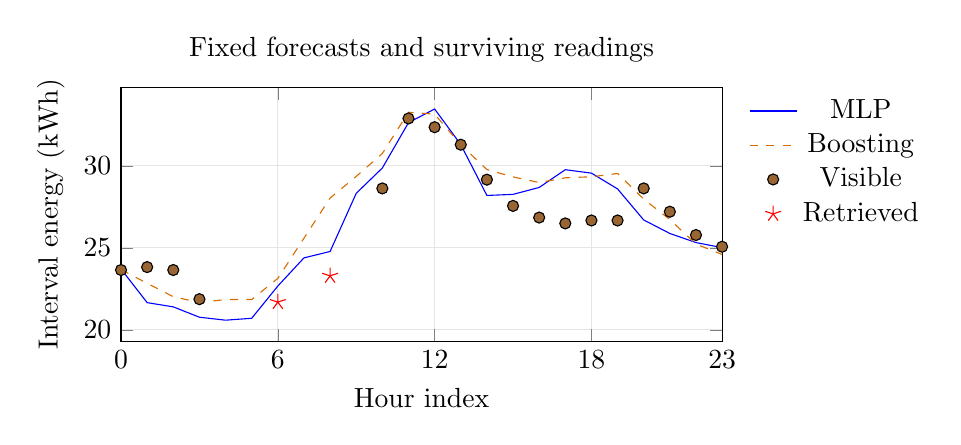
\begin{tikzpicture}
\begin{axis}[width=0.76\linewidth,height=4.8cm,tick label style={font=\normalsize},label style={font=\normalsize},legend style={font=\normalsize,draw=none},grid=major,grid style={gray!20},scaled ticks=false,xmin=0,xmax=23,xtick={0,6,12,18,23},xlabel={Hour index},ylabel={Interval energy (kWh)},legend pos=outer north east,title={Fixed forecasts and surviving readings}]
\addplot+[blue,mark=none] coordinates {(0,23.7089731) (1,21.65926053) (2,21.40056945) (3,20.76969428) (4,20.58918072) (5,20.7049956) (6,22.67158609) (7,24.38967792) (8,24.77970026) (9,28.32769632) (10,29.87362605) (11,32.63845034) (12,33.47187004) (13,31.30219642) (14,28.19734887) (15,28.26401218) (16,28.68569787) (17,29.76830032) (18,29.55914475) (19,28.59682085) (20,26.70253117) (21,25.87983072) (22,25.3235942) (23,25.0144397)};
\addlegendentry{MLP}
\addplot+[orange!85!black,mark=none,dashed] coordinates {(0,23.67335923) (1,22.83729057) (2,22.02153812) (3,21.666634) (4,21.84769547) (5,21.84769547) (6,23.13793853) (7,25.58930242) (8,28.04009073) (9,29.35798188) (10,30.76006346) (11,33.27016375) (12,33.15826742) (13,31.29274311) (14,29.77802672) (15,29.3296904) (16,28.98399795) (17,29.27340546) (18,29.33811927) (19,29.53693981) (20,27.97449045) (21,26.7313281) (22,25.23573177) (23,24.59836533)};
\addlegendentry{Boosting}
\addplot+[black,only marks,mark=*] coordinates {(0,23.64864865) (1,23.82645804) (2,23.64864865) (3,21.87055477) (10,28.62731152) (11,32.89473684) (12,32.36130868) (13,31.29445235) (14,29.16073969) (15,27.56045519) (16,26.84921764) (17,26.49359886) (18,26.67140825) (19,26.67140825) (20,28.62731152) (21,27.20483642) (22,25.78236131) (23,25.07112376)};
\addlegendentry{Visible}
\addplot+[red,only marks,mark=star,mark size=3pt] coordinates {(6,21.69274538) (8,23.29302987)};
\addlegendentry{Retrieved}
\end{axis}
\end{tikzpicture}

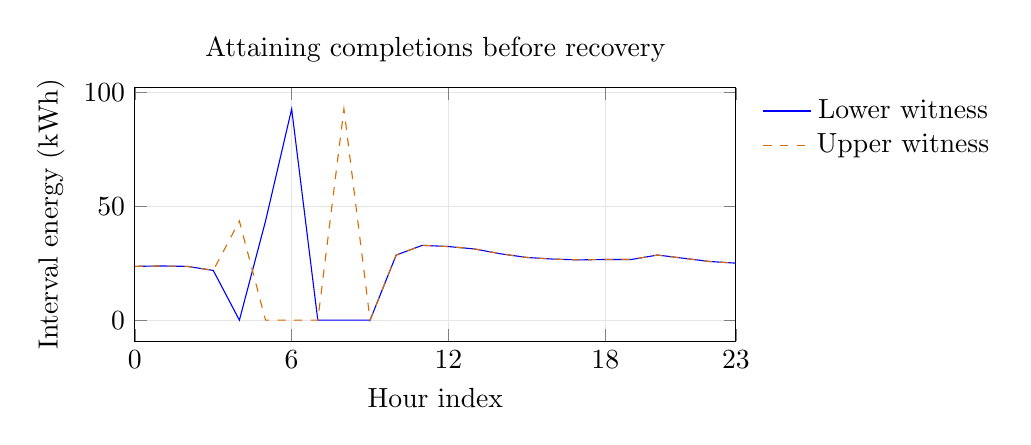
\begin{tikzpicture}
\begin{axis}[width=0.76\linewidth,height=4.8cm,tick label style={font=\normalsize},label style={font=\normalsize},legend style={font=\normalsize,draw=none},grid=major,grid style={gray!20},scaled ticks=false,xmin=0,xmax=23,xtick={0,6,12,18,23},xlabel={Hour index},ylabel={Interval energy (kWh)},legend pos=outer north east,title={Attaining completions before recovery}]
\addplot+[blue,mark=none] coordinates {(0,23.64864865) (1,23.82645804) (2,23.64864865) (3,21.87055477) (4,0) (5,43.56330014) (6,92.81650071) (7,0) (8,0) (9,0) (10,28.62731152) (11,32.89473684) (12,32.36130868) (13,31.29445235) (14,29.16073969) (15,27.56045519) (16,26.84921764) (17,26.49359886) (18,26.67140825) (19,26.67140825) (20,28.62731152) (21,27.20483642) (22,25.78236131) (23,25.07112376)};
\addlegendentry{Lower witness}
\addplot+[orange!85!black,mark=none,dashed] coordinates {(0,23.64864865) (1,23.82645804) (2,23.64864865) (3,21.87055477) (4,43.56330014) (5,0) (6,0) (7,0) (8,92.81650071) (9,0) (10,28.62731152) (11,32.89473684) (12,32.36130868) (13,31.29445235) (14,29.16073969) (15,27.56045519) (16,26.84921764) (17,26.49359886) (18,26.67140825) (19,26.67140825) (20,28.62731152) (21,27.20483642) (22,25.78236131) (23,25.07112376)};
\addlegendentry{Upper witness}
\end{axis}
\end{tikzpicture}

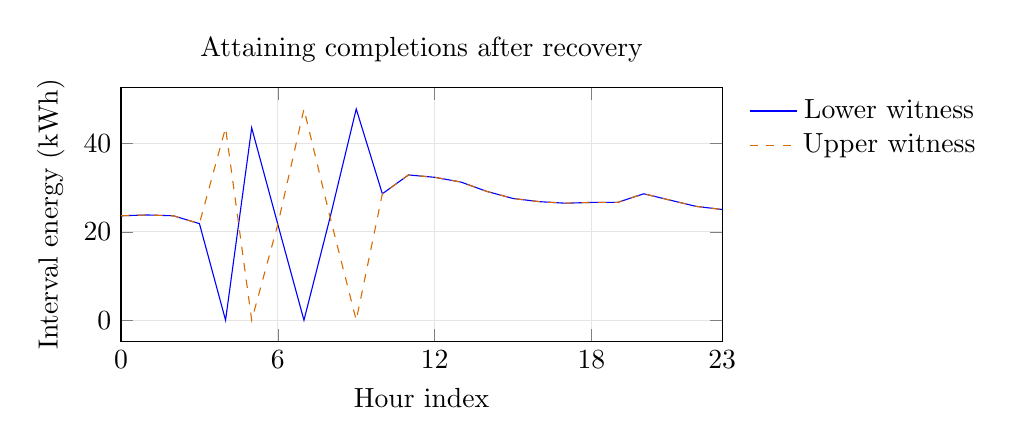
\begin{tikzpicture}
\begin{axis}[width=0.76\linewidth,height=4.8cm,tick label style={font=\normalsize},label style={font=\normalsize},legend style={font=\normalsize,draw=none},grid=major,grid style={gray!20},scaled ticks=false,xmin=0,xmax=23,xtick={0,6,12,18,23},xlabel={Hour index},ylabel={Interval energy (kWh)},legend pos=outer north east,title={Attaining completions after recovery}]
\addplot+[blue,mark=none] coordinates {(0,23.64864865) (1,23.82645804) (2,23.64864865) (3,21.87055477) (4,0) (5,43.56330014) (6,21.69274538) (7,0) (8,23.29302987) (9,47.83072546) (10,28.62731152) (11,32.89473684) (12,32.36130868) (13,31.29445235) (14,29.16073969) (15,27.56045519) (16,26.84921764) (17,26.49359886) (18,26.67140825) (19,26.67140825) (20,28.62731152) (21,27.20483642) (22,25.78236131) (23,25.07112376)};
\addlegendentry{Lower witness}
\addplot+[orange!85!black,mark=none,dashed] coordinates {(0,23.64864865) (1,23.82645804) (2,23.64864865) (3,21.87055477) (4,43.56330014) (5,0) (6,21.69274538) (7,47.83072546) (8,23.29302987) (9,0) (10,28.62731152) (11,32.89473684) (12,32.36130868) (13,31.29445235) (14,29.16073969) (15,27.56045519) (16,26.84921764) (17,26.49359886) (18,26.67140825) (19,26.67140825) (20,28.62731152) (21,27.20483642) (22,25.78236131) (23,25.07112376)};
\addlegendentry{Upper witness}
\end{axis}
\end{tikzpicture}
\caption{Frozen restricted-record daily evaluation; no saved-archive reconstruction. Worked historical audit, meter \texttt{MT\_002} on 2014-01-01. Lower and upper witnesses attain the bounds on MLP-minus-boosting MSE; they are measurement-compatible extremal completions, not predicted load profiles. The first chronologically unresolved eligible case was selected before inspecting the recovery outcome. Retrieved values come from the held-out reference trace. Full values and retained totals are in \texttt{study\_operator\_example.csv}.}
\label{fig:operator}\end{figure}

\FloatBarrier


\subsection{Restricted-record sensitivity}
The isolated daily-record experiment is a separate limited-input benchmark.
Appendices~\ref{app:restricted-daily} and~\ref{app:restricted-recovery}
retain its complete comparisons and budget grid. Its large recovery gains
must not be interpreted as gains after the saved archive has already been
used. The archive-consistent evidence above is the primary retrospective
application result.




\subsection{Attribution and the exact-versus-greedy distinction}
In the original restricted-record six-hour experiment, exact recovery exceeds
greedy certification by 1.15 percentage points on average across Portugal
meters. Exact alone certifies 785 dependent cases and greedy alone 119;
actual width is larger under exact recovery in 700 cases. Thus the worst-case
width optimum is not a pointwise certification optimum.
The preceding archive-consistent analysis isolates the much smaller
archive-aware allocator increment from free reconstruction and paid readings.
Appendix~\ref{app:greedy-detail} retains query counts, signed distributions
and descriptive bootstrap intervals.


\subsection{Total uncertainty and selective missingness}
Table~\ref{tab:sensitivity} retains every mask mechanism and total-error
setting for six missing targets and six-hour totals. Widening total
uncertainty enlarges the feasible set and cannot improve the mathematical
certificate. The contiguous, scattered, and highest-demand masks test
different locations of missing energy and forecast disagreement. The
highest-demand mask is an oracle stress condition, not a learned or
prospective outage predictor.
\begin{table}[htbp]
\centering\normalsize\setlength{\tabcolsep}{4pt}
\caption{Frozen restricted-record daily evaluation; no saved-archive reconstruction. Daily paired resolution (\%) with six missing targets and six-hour totals. High demand is an oracle stress mask. Every issued decision remained correct.}
\label{tab:sensitivity}
\begin{tabular}{llrrr}
\toprule
Source & Mask & Exact & $1\%$ & $5\%$\\
\midrule
Portugal & Contiguous & 18.8 & 18.1 & 15.8\\
Portugal & Scattered & 32.0 & 28.9 & 20.2\\
Portugal & High demand & 15.4 & 14.6 & 11.9\\
Household & Contiguous & 48.9 & 47.9 & 44.6\\
Household & Scattered & 67.8 & 65.2 & 57.0\\
Household & High demand & 32.5 & 31.6 & 27.3\\
Counters & Contiguous & 43.9 & 42.9 & 39.8\\
Counters & Scattered & 67.3 & 65.1 & 57.1\\
Counters & High demand & 35.8 & 34.7 & 30.3\\
\bottomrule
\end{tabular}
\end{table}

\FloatBarrier
\subsection{Numerical verification and execution cost}
The revised reference, integration, recovery, and malformed-input tests
passed. The study additionally passed 1,000
random study/reference cross-checks. Independent LP/QP audits and an
exhaustive adaptive-query oracle provide checks beyond the implementation's
own formulas. Their reports and source hashes accompany the manuscript.
The largest absolute LP discrepancy was $1.14\times10^{-13}$
across 1800 extrema; the corresponding
individual-error minimum discrepancy was $1.06\times10^{-9}$
across 600 constrained optimizations.
The adaptive oracle checked 5,952 finite small cases, including determined
last-coordinate queries and excess budgets, with exact agreement between
adaptive, exhaustive fixed-batch, and sorted-window optima.

On an Intel Core i7-8565U CPU with 15.75 GiB RAM, the revised main
pipeline took 809.8 s using two computation
threads and no GPU. Prepared-input timing used 30 feasible cases at each
length, five warmups, and three repetitions. The validated reference API
returned both extrema and witnesses in median 0.172 ms for
24 targets and 0.858 ms for 168 targets.
Two SciPy HiGHS calls on prepared matrices took
5.151 and
5.954 ms, respectively.
These measurements include solver-call overhead and exclude fitting and
file processing. They describe one host under uncontrolled concurrent
activity; no end-to-end forecasting speedup is inferred.

The additional two-query batch optimizer was timed on 30 prepared
24-target problems at each gap size, with five warmups and three repeats.
Its median latency was 0.057 ms for
six missing targets and 0.058 ms for
twelve. This measures query selection alone; input preparation, retrieval
from a real meter or archive, and recomputation of the bounds are excluded.
The experiment does not measure communication latency.

The separate interval-total batch solver was checked on 86
small synthetic instances by enumerating 1,247
query subsets and computing extrema using 3,458
HiGHS linear-program solves. It also passed 482
conditional-answer checks, 108
reductions to the exact-total implementation, and 25
invalid-input checks. The maximum recorded discrepancy was zero in these
constructed cases; this is finite numerical verification, not an
outward-rounded arithmetic guarantee. This extension was not used to
replace or pool the primary exact-total meter results, and its tests do
not measure field deployment benefits.
\FloatBarrier

\subsection{Replication and total-uncertainty sensitivity}
The frozen additional 30-consumer panel increases restricted-record
certification from 25.02\% to 64.11\% with exact two-query recovery;
archive-aware certification instead starts at 96.87\% and reaches 98.57\%.
The archive-aware exact-over-greedy increment is 0.061 percentage points
(Appendix~\ref{app:replication-results}). This supports repeatability within
the same dataset and calendar, not independent infrastructure validation.
With constructed $\pm5\%$ total bands on the original Portugal traces,
certification increases from 15.8\% to 46.3\% under restricted access and
from 96.5\% to 98.1\% with the saved archive. Appendix~\ref{app:interval-results}
retains every cohort, tolerance and policy result.


\subsection{Exact randomized recovery: robust gain and realized tradeoff}
\label{sec:random-results}
Of the 20,736 fixed comparisons, 1,074 retain positive width after free
archive information and total deductions. The finite-game solutions have
2,341 positive-probability batches. Independent reconstruction checks all
20,736 cases, all positive batches, 19,662 permitted direct target copies,
and all 1,074 compact-versus-finite-game optima. The largest objective
discrepancy, divided by $\max(1,\text{initial width})$, is
$1.34\times10^{-13}$. No issued support-batch certificate contradicts
the reference comparison. These dependent checks validate the calculation;
their count is not an independent statistical sample size.

Table~\ref{tab:random-results} separates the robust objective from realized
outcomes. Portugal's mean normalized worst expected width decreases from
29.595\% to 26.673\% of its initial width, a relative reduction of 9.88\%
against the exact deterministic optimum. Its normalized expected width at
the actual record increases from 20.154\% to 23.670\%, or 17.45\% relatively.
The household reductions and increases are 6.66\% and 11.05\%, respectively.
Certification decreases slightly in both cohorts. The robust objective
improves strictly in 663 positive-width cases; realized expected width
improves in 14, worsens in 649, and is unchanged in the remaining 411.
No query-count advantage is claimed: both exact policies use two readings
in these positive-width cases.

\begin{table}[htbp]\centering\small
\caption{Six-hour contiguous gaps, exact six-hour totals, seed 1103, and $B=2$ per day/model pair. Randomized and deterministic exact recovery under identical saved-archive
access and budget. Width columns are percentages of initial width: first sum
within each meter, then average meter ratios. Certification averages all
day--pair cases within each meter, then meters. ``Rand.'' reports expectations
over the optimized batch distribution. Lower width is better; higher
certification is better.}\label{tab:random-results}
\begin{tabular}{lrrrrrr}\toprule
&\multicolumn{2}{c}{Worst width}&\multicolumn{2}{c}{Realized width}&\multicolumn{2}{c}{Certification (\%)}\\
Cohort&Det.&Rand.&Det.&Rand.&Det.&Rand.\\\midrule
Portugal & 29.595 & 26.673 & 20.154 & 23.670 & 98.795 & 98.688 \\
Household & 22.038 & 20.570 & 14.143 & 15.706 & 98.848 & 98.734 \\
\bottomrule\end{tabular}\end{table}

This adverse realized tradeoff is consistent with the objective: minimizing
the largest expected ambiguity over all compatible records does not
minimize width or maximize certification at the particular realized load
profile. Randomization is therefore a robust-design option, not an
empirically dominant default replacement for deterministic recovery.

The compact implementation agrees with exhaustive finite-game programs on
all 42 synthetic cases to within $1.78\times10^{-13}$ absolute objective
error. Constructed $(m,r)=(4,2),(6,2),(9,3),(12,2)$ instances attain factors
2, 3, 3, and 6, respectively. These are sharpness examples, not estimates
of typical field gains. Table~\ref{tab:compact-scale} demonstrates that the
implementation need not enumerate all batches. The larger instance has
more than 3.65 billion size-six subsets but only 3,221 LP variables.
The independent sampler audit also checks its induced mixture, rather than
only whether sampled batches have the correct size: the largest recovered
coefficient discrepancy is $1.78\times10^{-15}$. All floating-point
projection and normalization corrections are recorded in Online Resource~1.

\begin{table}[htbp]\centering\small
\caption{Fixed one-block scalability checks. The batch counts are combinatorial
counts, not enumerated runs. LP variable counts include the epigraph. These
two synthetic configurations establish feasibility at these sizes, not an
asymptotic runtime benchmark.}\label{tab:compact-scale}
\begin{tabular}{rrrr}\toprule
Coordinates $m$&Budget $B$&Size-$B$ batches&Compact LP variables\\\midrule
60 & 4 & 487,635 & 846 \\
120 & 6 & 3,652,745,460 & 3,221 \\
\bottomrule\end{tabular}\end{table}


\subsection{Secondary optimization does not remove the observed penalty}
\label{sec:tie-results}
All 2,148 secondary LPs complete. Neither the dominance refinement nor the
uniform-completion refinement changes the realized expected width in any
of the 1,074 positive-width cases beyond the declared $10^{-9}$ scaled
comparison tolerance. Neither strictly improves the secondary objective at
that tolerance. The largest normalized primary lower-bound gap is
$1.96\times10^{-12}$ and the largest dominance residual is
$5.75\times10^{-12}$. Portugal's normalized expected width remains
23.670\% for both refinements, versus 20.154\% for deterministic recovery;
certification remains 98.688\% versus 98.795\%. The household summaries
are likewise unchanged at the displayed precision. Independent replay checks
every refined distribution, secondary optimum, and case aggregation.
Thus the reported 17.45\% Portugal penalty persists under these specified
target-independent tie refinements. It is not evidence that every minimax
policy has that penalty, or that the percentage transfers to other records.
The exact counterexample in Section~\ref{sec:tie-selection} remains a useful
regression test even though this empirical panel shows no such improvement.

\subsection{Randomized recovery on additional consumers}
We subsequently froze the uniform-barycenter secondary rule and applied it to the existing 30-consumer Portugal replication: all 3,210 meter-days and all six model pairs (19,260 cases), without refitting. The information regime used the same six-hour contiguous mask, seed 1103, exact six-hour totals, saved persistence copies, exact-total closure, and budget $B=2$. Masked observations and measurement totals were first exported to a selection-only archive. A separate process optimized policies from these inputs, without opening the reference-target archive; the policies were hashed before realized-performance evaluation. This is a post-review audit of an existing held-out-consumer archive, not a prospective study or a new data source.

Of the 19,260 cases, 899 retained positive width after free reconstruction and closure; all were evaluated. Every positive-width case passed both the finite-game primal--dual checks and a comparison with the compact formulation, with maximum normalized objective discrepancy $6.94\times10^{-14}$. The independent arithmetic replay checked archive reconstruction, selected-batch interval containment, query budgets, and the saved primary dual bounds. All 3,958 positive-probability batches across the secondary policy and the original primary optimizer passed containment checks.

The adverse realized-performance result persisted. Consumer-macro worst-width fractions were 0.28112 for deterministic recovery and 0.25501 for the secondary randomized policy; realized-width fractions were 0.18497 and 0.21935, respectively. These fractions divide each consumer's summed posterior widths by its summed initial width, then average over consumers. All-case certification was 98.894\% versus 98.776\%, and positive-width-case certification was 76.318\% versus 73.798\%; these are consumer-macro averages of case-level certification probabilities. Mean paid queries were equal to the displayed precision: 0.09330 over all cases and 1.99885 in the positive-width stratum. Among the 899 positive-width cases, randomization strictly reduced worst width in 564; its realized width improved in 12, worsened in 553, and tied in 334 relative to deterministic recovery. The original primary optimizer gave the same aggregate results at the displayed precision. Thus the frozen secondary criterion did not remove the practical tradeoff on these additional consumers.

\subsection{Computational scaling of randomized recovery}

We froze 28 synthetic cases before optimization: the full factorial $G\in\{1,2,4\}$, $m\in\{6,12\}$, $B=\lfloor Gmf\rfloor$, $f\in\{1/4,1/2\}$, and two coefficient/total profiles, plus four single-block cases with $m\in\{24,48\}$ and $f=1/2$. The profiles were distinct coefficients with homogeneous totals, and threefold coefficient ties with geometric coefficient scales and heterogeneous totals. Thus ties and heterogeneity vary jointly; the comparison does not isolate either effect. The manifest fixes every coefficient, total, seed, budget, and exhaustive-solver eligibility decision.

Each method/case ran once in a fresh subprocess on an Intel Core i7-8565U (four physical cores, 16.9 GB RAM), Windows 11, Python 3.12.14, NumPy 2.5.3, and SciPy 1.18.1. HiGHS and numerical-library thread limits were one. Method time includes LP construction, solution, and policy compilation after imports; separately measured diagnostic overhead is removed. Peak working set is the worker-reported whole-process peak, including interpreter and imports. The wall limit was 20 s. A parent memory watchdog used a 1 GiB threshold, but the Windows environment launcher can make that watchdog observe the redirector; therefore it is not a verified worker allocation cap. Every worker-reported peak was below 169 MiB. Runs were sequential on a shared host, without timing repetitions.

All 28 compact runs returned an optimal LP and passed 560 seeded exact-budget/sample-identity checks. Maximum normalized primal violation, stationarity residual, and primal--dual gap were $3.78\times10^{-15}$, $5.22\times10^{-15}$, and $5.78\times10^{-16}$, respectively; the recorded dual sign violation was zero. Exhaustive finite-game comparison was prescribed only for at most 25,000 admissible batches and at most 100,000 prefilter Cartesian-product candidates. All 12 eligible comparisons ran, with maximum objective discrepancy $1.27\times10^{-15}$ after division by $\max(1,W_0)$; the other 16 were retained as predetermined skips. There were no timeouts, solver errors, or memory terminations.
Table~\ref{tab:compact-scaling-audit} reports both profiles at every dimension/budget setting. Its ranges span two different instances, not repeated-run uncertainty. Full per-case objectives, sparse dimensions/nonzeros, timings, memory, and numerical diagnostics are archived. These bounded measurements establish operability at the sampled sizes; they do not establish runtime dominance or empirical asymptotic complexity, and the residual checks are floating-point evidence rather than exact certificates.
\begin{table}[htbp]
\centering\small
\caption{Frozen compact-policy scaling audit. Each row contains two coefficient/total profiles; all runs succeeded. Time and peak-memory ranges span those profiles. Vars. is the LP variable count; Finite is the number of prescribed exhaustive comparisons completed.}
\label{tab:compact-scaling-audit}
\begin{tabular}{rrrrrrr}
\hline
$G$ & $m$ & $B$ & Vars. & Method time (s) & Peak (MiB) & Finite \\
\hline
1 & 6 & 1 & 14 & 0.010--0.015 & 71.4--71.7 & 2/2 \\
1 & 6 & 3 & 31 & 0.011--0.019 & 71.5--71.5 & 2/2 \\
1 & 12 & 3 & 91 & 0.012--0.014 & 71.8--71.8 & 2/2 \\
1 & 12 & 6 & 197 & 0.014--0.023 & 72.0--72.1 & 2/2 \\
2 & 6 & 3 & 142 & 0.013--0.024 & 71.9--71.9 & 2/2 \\
2 & 6 & 6 & 164 & 0.020--0.022 & 72.1--72.1 & 2/2 \\
2 & 12 & 6 & 1,346 & 0.091--0.127 & 75.7--76.1 & 0/2 \\
2 & 12 & 12 & 2,974 & 0.246--0.594 & 80.2--80.4 & 0/2 \\
4 & 6 & 6 & 946 & 0.042--0.053 & 74.2--74.2 & 0/2 \\
4 & 6 & 12 & 1,162 & 0.047--0.069 & 74.8--74.8 & 0/2 \\
4 & 12 & 12 & 22,538 & 3.356--4.056 & 126.3--126.8 & 0/2 \\
4 & 12 & 24 & 38,820 & 9.933--10.012 & 160.5--168.6 & 0/2 \\
1 & 24 & 12 & 1,366 & 0.091--0.105 & 75.6--75.7 & 0/2 \\
1 & 48 & 24 & 10,076 & 0.606--1.631 & 97.3--97.3 & 0/2 \\
\hline
\end{tabular}
\end{table}

% Standalone integration fragment, based on panel_summary.json and immutable
% recorded source/decode snapshots. Does not claim natural hidden-label truth.
\subsection{Natural precipitation accumulations: a zero-query audit}
\label{sec:noaa-natural}
The aggregate-only information structure also occurs without deliberately
removing fine-resolution labels. NOAA's COOP Hourly Precipitation Data retain
legacy records in which an accumulation total is reported but its distribution
over the intervening hours is unavailable \cite{noaa_hpd_v2,noaa_hpd_format}.
This supports a limited retrospective verification task: determine whether two
fixed forecasts can be ordered for every temporal allocation consistent with
the archived total. It does not establish that historical hourly readings can
be recovered, or assign a cost to recovering them.

We fixed a small source-based panel before inspecting forecast comparisons.
A lexical screen of the first three CONUS station files found nine simple
one-day accumulation records after 2000 at Alberta, Alabama
(USC00010140; $32.2322^{\circ}$N, $87.4104^{\circ}$W). All nine occur in December
2008 or June 2009 and are retained. We also retain every eligible complete day
in those two months. Of 61 calendar dates, 52 are included: nine accumulation
days and 43 complete days. Seven dates have no hourly row, and two contain
multi-day accumulations outside this fixed one-day design. Selection is
purposive and does not estimate the prevalence of useful coarse records.

On each natural case, the hourly record has a beginning flag at 00:00,
interior accumulation flags, and an ending flag with the total at 23:00.
The current CSV definition assigns these fields to $[00{:}00,01{:}00)$ and
$[23{:}00,24{:}00)$ local standard time, respectively. Thus the constraint
covers the full 24-hour recorded day. Values in hundredths of an inch are
converted to millimetres by multiplication by $0.254$. We use the original
accumulation total, never the computed \texttt{DlySum} field as an independent
measurement. The station inventory specifies UTC$-6$ in both months.

The permitted public-source audit includes the parallel 15-minute station
file and the digital raw-data files for both months. For the six December
cases, the parallel file supplies three initial zero quarter-hours followed
by the same unresolved accumulation and matching total. The three June
event dates are absent. No selected station record is present in either
monthly digital raw file. These findings are preserved with source-row
pointers and hashes. Initial zero quarter-hours do not identify any complete
three-hour target: every three-hour bin still contains unconstrained
nonnegative periods, so projecting the checked information onto the eight
bins leaves $y\geq0$ and $\sum_i y_i=T$. Several legacy download endpoints
returned HTTP 404; the conclusion concerns the documented files checked,
not a proof that no other archive exists.

We compare the GEFSv12 control member with the fixed arithmetic mean of its
five daily members, with no fitting or member selection
\cite{guan2022gefs,noaa_gefs_archive}. These are retrospective numerical
weather forecasts, not forecasts issued in 2008--2009 or an ML-performance
benchmark. The nearest $0.25^{\circ}$ grid point is 8.6565\,km from the station.
The nominal cycle is 00:00 UTC; Phase 2 integration actually starts at 03:00
UTC following the replay analysis. Guan et al.'s documented corrections
concern the initial 00:00--03:00 and 00:00--06:00 accumulated fields. We use
valid windows 06:00--06:00 the following day, checked against GRIB validity
metadata, corresponding to eight local three-hour bins. Nested three- and
six-hour precipitation fields are differenced. There were 28 negative
differences, between $-0.05$ and $-0.01$\,mm,
across 27 of 260 member-days. Each discrepancy passed the recorded packing
resolution bound; this establishes consistency with differential quantization,
not its exclusive causal explanation. Our specified nonnegative preprocessing caps the first
three-hour amount at its six-hour total and uses the residual for the second,
preserving every decoded six-hour total. All raw differences and the complete
raw-versus-processed endpoint sensitivity are retained.

Let $a$ denote the processed control and $b$ the processed ensemble mean.
For the daily mean squared-error contrast $\Delta=L(a)-L(b)$, the direct
paired bounds are compared with subtraction of separately sharp individual
MSE bounds using exactly the same information. Table~\ref{tab:noaa-natural}
reports all nine natural cases. Two days certify lower ensemble-mean MSE;
the separate individual bounds certify neither. One day is an exact forecast
tie and six permit both orderings. Uniform allocation gives point orderings
on all eight non-tie days, but six of those orderings are not implied by the
observed information. There is no fine-resolution truth with which to label
those point decisions correct or incorrect.

\begin{table}[t]
\centering
\caption{All natural accumulation cases. Bounds are for control minus
ensemble-mean MSE over eight three-hour bins, in $\mathrm{mm}^2$.
Positive intervals certify the ensemble mean.}
\label{tab:noaa-natural}
\begin{tabular}{lrrrl}
\hline
Date & Total (mm) & Lower & Upper & Conclusion\\
\hline
2008-12-05 & 12.700 & 0.00000 & 0.00000 & exact tie\\
2008-12-10 & 12.700 & 7.18081 & 25.37356 & ensemble\\
2008-12-11 & 33.020 & $-24.65680$ & 26.47467 & unresolved\\
2008-12-17 & 5.080 & $-0.48739$ & 0.43971 & unresolved\\
2008-12-28 & 5.080 & $-1.01836$ & 0.37356 & unresolved\\
2008-12-29 & 5.080 & $-0.04186$ & 0.03942 & unresolved\\
2009-06-05 & 7.874 & $-1.15768$ & 1.48011 & unresolved\\
2009-06-14 & 1.524 & 0.64919 & 1.47063 & ensemble\\
2009-06-24 & 9.652 & $-0.00005$ & 0.04821 & unresolved\\
\hline
\end{tabular}
\end{table}

The conclusions on all nine natural days are unchanged using raw signed
increments; preprocessing changes two dry-control conclusions to ties.
All 43 complete controls have zero recorded precipitation, predominantly
archive-assigned zero flags. Their feasible sets are singleton zero vectors,
so they test only this degenerate case and do not validate nonzero natural
endpoints against hidden truth. Combining their observed loss contrasts with
the nine natural intervals yields the 52-day interval
$[-0.250924,1.195845]\,\mathrm{mm}^2$, which does not order the forecasts.
We also fixed a supplementary $\pm2.54$\,mm total perturbation before inspecting
paired outcomes, motivated by NOAA's nominal $0.1$-inch gauge accuracy.
With $T\in[\max(0,T_0-2.54),T_0+2.54]$, only the 2008-12-10 strict certificate
remains. This is a source-inspired sensitivity, not a validated error bound
for the legacy totals or a confidence statement about physical rainfall.

This panel supplies a concrete natural use of zero-query partial-label
evaluation: some forecast comparisons are identifiable even when their
individual scores are not. Its scope is limited by the nine selected events,
recording and measurement uncertainty, and grid-point versus gauge
representativeness. It provides neither evidence of retrieval savings nor
a general ranking of the forecast systems. The lightweight archive contains
source excerpts, every decoded-message record and provenance pointer, both
forecast variants, and an offline executable reconstruction; fresh GRIB
decoding and full-source checks are distinguished from excerpt arithmetic.

\section{Discussion}
The methodological result is exact optimization of the uncertainty left in
a fixed-record model comparison. Shared-target cancellation makes the
comparison linear; sorted windows solve deterministic recovery; weighted
endpoints and a compact flow representation make randomized batch recovery
tractable without enumerating its query subsets. The deterministic adaptivity
identity and sharp one-block randomization gap characterize what these
policies can guarantee. The synthetic scaling study establishes operability
across the reported sizes and budgets, while retaining the limits of its
single-run timing and memory measurements.

For an applied evaluator, the comparison interval can accompany an existing
imputed score. If it excludes zero, the ordering is supported by every
completion in the declared set; if it straddles zero, witness completions
show exactly why the available information does not determine the winner.
This distinction matters even when an imputer performs well on the observed
record. The historical donor makes no full-period errors in the reported
archive-aware exact-total grid at full coverage. The experiment therefore
supports a conditional defensibility guarantee, not superiority in observed
whole-period ranking accuracy. The conservative selector likewise has worse
Portugal mean normalized realized regret than the donor (1.549 versus 0.195,
both multiplied by $10^3$); Appendix~\ref{app:regret} retains the complete
tradeoff.

The information available to the evaluator determines how much recovery
can add. Later persistence forecasts directly reveal most masked energy
targets in this historical archive. The large restricted-record recovery
gains describe a different information set; after free reconstruction,
the exact allocator's certification increment over greedy is small.
The additional-consumer analyses reproduce this distinction within the
same source and calendar. Their contribution is evidence about the fixed
procedure, rather than a measurement of field outage prevalence or
production retrieval costs.

Randomization improves worst expected width but does not improve the
observed energy-audit outcomes. The adverse width and certification results
persist under the two specified secondary refinements and the fixed-rule
additional-consumer audit. Section~\ref{sec:tie-selection} explains why a
minimax policy must specify its secondary selection; the contrast family
that follows shows how the same robust policy can help or harm at different
feasible records. Randomized recovery is consequently appropriate when
worst expected ambiguity is the stated objective, not an empirically
dominant replacement for deterministic recovery or imputation.

The rainfall application establishes a narrower positive use: two of nine
naturally accumulated daily records support a strict forecast comparison,
although separately bounded individual scores do not. One survives the
declared total sensitivity. The six ambiguous cases, one exact tie and
unresolved combined-period result remain part of that evidence. The 43
dry controls validate only a degenerate observation case. These records
support zero-query identification without establishing recoverable missing
hourly truth, a general forecast ranking, or a benefit from paid recovery.

\subsection{Operational interpretation}
An operational audit must declare its target window, information cutoff,
prediction archive, observed values and aggregate constraints. Verified
direct target copies and aggregate-determined values are incorporated
before comparing models or selecting queries. The evaluated energy regime
uses documented persistence copies; it does not invert the other fitted
predictors or use unsaved feature caches. Sharpness is relative to this
declared set, not to every possible record in the forecasting system.

If the comparison remains unresolved and a separate source can supply
individual readings, the evaluator can select a batch, validate the returned
values, update residual totals and recompute the interval. The budget is
per model pair and counts readings, not network transactions or staff time.
It provides no retrieval saving when an entire gap is obtained at the same
cost. Shared requests across many pairs, cancellation after an early decision,
and optimal randomized adaptive recovery require different objectives and
evaluations. Actual target-arrival and repair timestamps are absent here,
so decision latency and deployment savings remain unmeasured.

\subsection{Limitations and scope}
The guarantees depend on the measurement model. Energy outages are imposed
retrospectively; UCI totals are constructed from complete traces, and retained
BLEM counter endpoints do not demonstrate an independent backup channel's
survival. Complete-record eligibility, the convenience sample and historical
test calendars limit generalization. The fixed MLP and other forecasters
define reproducible comparisons, rather than state-of-the-art accuracy.
Post-review analyses reuse these records and are not independent prospective
cohorts. Constructed tolerance bands are sensitivity assumptions, not
calibrated measurement-error distributions.

Nonnegative uncapped targets and disjoint totals permit the exact recovery
reductions. Physical caps, overlapping or correlated totals, signed flows,
unequal query costs and uncertain returned readings require their own
constraints and algorithms; the randomized results here use exact totals.
Other losses need not retain squared-error cancellation. Mathematical
sharpness does not validate the measurements, and binary64 checks do not
supply outward-rounded machine-certified enclosures.

\FloatBarrier
\section{Conclusion}
Aggregate observations support sharp comparisons of fixed forecasts despite
missing verification targets. For deterministic recovery, sorted windows
and dynamic programming solve the worst remaining width objective, and
deterministic adaptation cannot improve it. For randomized nonadaptive
recovery, weighted endpoints and a compact budget-flow formulation solve
the worst expected width objective without enumerating query subsets.
For positive optima and $r\geq2$, the one-block deterministic-to-randomized ratio is bounded by $m/r$, with
attaining clustered examples when $r$ divides $m$.

The experiments distinguish these guarantees from realized performance.
The archive-consistent energy audit uses permitted direct target copies
before evaluating every comparator. Randomization improves its optimized
robust objective but has an unfavorable realized tradeoff on the tested
energy panel. Naturally accumulated rainfall records support two strict
daily comparisons from surviving totals, with one robust to the specified
total sensitivity. The practical output is an auditable interval, a decision
when justified, and an exactly optimized recovery policy for the selected
criterion. Operational retrieval costs and arrival times remain unmeasured.

\FloatBarrier
\appendix
\section{Additional Designs, Extensions, and Energy Results}\label{app:additional}
This appendix retains the supporting designs and complete analyses. The
original uniform-random retrieval baseline in its tables is distinct from
the optimized batch distribution of Section~\ref{sec:randomized-recovery}.
\subsection{Daily decisions and the value of pairing}\label{app:restricted-daily}
For two missing hours and exact six-hour totals, paired resolution was
71.5\%, 91.8\%, 91.8\% for Portugal, the household,
and the counter cohort, respectively; separate individual-error bounds
resolved 21.9\%, 62.7\%, 61.6\%. At six missing
hours the corresponding paired rates were 18.8\%, 48.9\%, 43.9\%,
versus 1.9\%, 8.6\%, 8.6\% for separate bounds.
The Portugal six-hour-gap gain was 16.9
percentage points (descriptive whole-meter bootstrap 95\% interval:
13.7--20.1).
Both methods receive identical measurements. Their difference therefore
isolates the benefit of comparing against the shared unknown target.

The profile imputer made daily ordering errors of
4.6\%, 3.5\%, 4.5\% in that setting, while deciding
100.0\%, 100.0\%, 100.0\% of comparisons.
Certified decisions trade coverage for a conditional all-completions
guarantee; these figures alone do not establish error-rate superiority
at equal coverage. With twelve missing hours and only a daily total,
paired resolution fell to 2.8\%, 3.7\%, 4.7\%.
The complete contiguous-gap grid is retained in Table~\ref{tab:daily}.
\begin{table*}[htbp]
\centering\normalsize\setlength{\tabcolsep}{4pt}
\caption{Frozen restricted-record daily evaluation; no saved-archive reconstruction. Daily comparison results for contiguous gaps and exact totals. Gap and total are hours. Paired and Separate columns give resolved comparisons (\%); the four point-method columns give errors among decisions (\%). Both bounding methods made zero incorrect decisions. Point methods make nearly all decisions; their higher coverage must be considered when comparing errors. Rates are macro-averaged over meters. Unresolved fraction is 100 minus resolved percentage.}
\label{tab:daily}
\begin{tabular}{lrrrrrrrr}
\toprule
Source & Gap & Total & Paired & Separate & Deletion & Uniform & Profile & Donor\\
\midrule
Portugal & 2 & 6 & 71.5 & 21.9 & 4.1 & 1.3 & 0.9 & 0.9\\
Portugal & 2 & 24 & 66.4 & 8.9 & 4.1 & 1.6 & 1.1 & 1.1\\
Portugal & 6 & 6 & 18.8 & 1.9 & 10.3 & 7.5 & 4.6 & 5.0\\
Portugal & 6 & 24 & 13.5 & 1.3 & 10.3 & 10.5 & 6.2 & 6.4\\
Portugal & 12 & 6 & 5.8 & 0.6 & 20.2 & 13.5 & 8.0 & 9.6\\
Portugal & 12 & 24 & 2.8 & 0.3 & 20.2 & 21.0 & 13.0 & 13.9\\
Household & 2 & 6 & 91.8 & 62.7 & 4.5 & 0.9 & 0.8 & 1.1\\
Household & 2 & 24 & 90.3 & 56.2 & 4.5 & 1.2 & 1.0 & 1.3\\
Household & 6 & 6 & 48.9 & 8.6 & 10.7 & 4.6 & 3.5 & 5.5\\
Household & 6 & 24 & 34.8 & 4.9 & 10.7 & 7.5 & 5.4 & 7.2\\
Household & 12 & 6 & 13.0 & 0.4 & 20.0 & 8.6 & 7.2 & 10.1\\
Household & 12 & 24 & 3.7 & 0.0 & 20.0 & 15.3 & 13.0 & 16.6\\
Counters & 2 & 6 & 91.8 & 61.6 & 4.0 & 1.0 & 0.7 & 0.8\\
Counters & 2 & 24 & 89.7 & 53.5 & 4.0 & 1.1 & 0.9 & 1.1\\
Counters & 6 & 6 & 43.9 & 8.6 & 11.8 & 5.6 & 4.5 & 5.3\\
Counters & 6 & 24 & 30.6 & 4.9 & 11.8 & 7.4 & 5.7 & 6.8\\
Counters & 12 & 6 & 11.6 & 1.7 & 24.3 & 11.2 & 8.7 & 11.4\\
Counters & 12 & 24 & 4.7 & 0.3 & 24.3 & 17.4 & 12.7 & 16.3\\
\bottomrule
\end{tabular}
\end{table*}

\FloatBarrier

\subsection{Budgeted recovery of measured values}\label{app:restricted-recovery}
Table~\ref{tab:recovery} reports the complete recovery grid. For six-hour
gaps, allowing two selected readings per pair raised paired resolution
from 18.8\%, 48.9\%, and 43.9\% to
60.1\%, 89.2\%, and 86.9\% for Portugal,
the household, and the counter cohort, respectively. The recovered values
are actual withheld readings; no synthetic completion is substituted for
them. All newly certified decisions remained correct.

The optimal rule left 28.6\%, 25.7\%, and 23.5\% of
the initial worst-case width at that budget, compared with
31.0\%, 28.1\%, and 25.3\% for greedy width
reduction. The implementation checked on every comparison that the
optimal batch's worst-case width was no larger than each baseline's and
that the realized post-recovery width was within its predicted bound.
These are the optimized criterion and its direct numerical verification.
Table~\ref{tab:width} reports the width comparison across gap sizes;
Appendix~\ref{app:neural-pairs} also displays coverage and worst-case width across budgets.
\begin{table*}[htbp]
\centering\normalsize\setlength{\tabcolsep}{4pt}
\caption{Frozen restricted-record daily evaluation; no saved-archive reconstruction. Completed recovery experiment: exact six-hour totals, three mask seeds, pair-specific batch queries. All six policy columns are final resolution (\%), macro-averaged over meters. Wt.: weighted sampling without replacement, using prediction-only contrast weights inspired by active comparison. Every certificate was correct. Optimal refers to worst-case width, not a guarantee of maximum empirical resolution. All policies use at most the listed number of recovered targets.}
\label{tab:recovery}
\begin{tabular}{lrrrrrrrr}
\toprule
Source & Gap & Budget & Optimal & Greedy & Uniform random & Max. $|c|$ & Wt. $|c|$ & Wt. $c^2$\\
\midrule
Portugal & 6 & 0 & 18.8 & 18.8 & 18.8 & 18.8 & 18.8 & 18.8\\
Portugal & 6 & 1 & 35.1 & 35.1 & 25.3 & 30.5 & 26.4 & 27.7\\
Portugal & 6 & 2 & 60.1 & 58.9 & 36.8 & 48.0 & 40.3 & 43.1\\
Portugal & 6 & 3 & 86.1 & 85.2 & 57.0 & 71.9 & 63.4 & 67.3\\
Portugal & 12 & 0 & 5.8 & 5.8 & 5.8 & 5.8 & 5.8 & 5.8\\
Portugal & 12 & 1 & 9.2 & 9.2 & 6.7 & 8.0 & 6.9 & 7.2\\
Portugal & 12 & 2 & 14.2 & 13.8 & 8.1 & 10.9 & 8.6 & 9.4\\
Portugal & 12 & 3 & 21.6 & 20.3 & 9.8 & 14.9 & 11.1 & 12.4\\
Household & 6 & 0 & 48.9 & 48.9 & 48.9 & 48.9 & 48.9 & 48.9\\
Household & 6 & 1 & 73.0 & 73.0 & 58.8 & 66.7 & 61.3 & 63.3\\
Household & 6 & 2 & 89.2 & 88.3 & 71.1 & 81.7 & 75.8 & 78.2\\
Household & 6 & 3 & 97.1 & 96.6 & 84.7 & 93.1 & 88.7 & 90.3\\
Household & 12 & 0 & 13.0 & 13.0 & 13.0 & 13.0 & 13.0 & 13.0\\
Household & 12 & 1 & 28.3 & 28.3 & 16.6 & 23.0 & 18.2 & 19.8\\
Household & 12 & 2 & 44.6 & 43.5 & 21.8 & 34.0 & 25.2 & 28.3\\
Household & 12 & 3 & 60.8 & 58.5 & 28.1 & 46.7 & 33.5 & 38.7\\
Counters & 6 & 0 & 43.9 & 43.9 & 43.9 & 43.9 & 43.9 & 43.9\\
Counters & 6 & 1 & 70.2 & 70.2 & 55.7 & 65.2 & 58.5 & 61.5\\
Counters & 6 & 2 & 86.9 & 86.2 & 67.3 & 80.5 & 73.8 & 77.5\\
Counters & 6 & 3 & 96.7 & 96.5 & 82.6 & 91.9 & 87.2 & 89.9\\
Counters & 12 & 0 & 11.6 & 11.6 & 11.6 & 11.6 & 11.6 & 11.6\\
Counters & 12 & 1 & 26.0 & 26.0 & 15.0 & 22.1 & 16.8 & 19.5\\
Counters & 12 & 2 & 40.8 & 39.4 & 19.8 & 32.4 & 23.9 & 27.2\\
Counters & 12 & 3 & 56.2 & 53.2 & 25.2 & 43.9 & 31.9 & 36.7\\
\bottomrule
\end{tabular}
\end{table*}
\begin{table*}[htbp]
\centering\normalsize\setlength{\tabcolsep}{4pt}
\caption{Frozen restricted-record daily evaluation; no saved-archive reconstruction. Remaining worst-case width (\% of initial width) with budget two. Within each meter, total remaining width is divided by total initial width; ratios are then macro-averaged. This is the objective optimized by the proposed recovery rule.}
\label{tab:width}
\begin{tabular}{lrrrrrrr}
\toprule
Source & Gap & Optimal & Greedy & Uniform random & Max. $|c|$ & Wt. $|c|$ & Wt. $c^2$\\
\midrule
Portugal & 6 & 28.6 & 31.0 & 72.7 & 46.8 & 63.1 & 57.2\\
Portugal & 12 & 52.8 & 54.9 & 89.5 & 69.4 & 84.4 & 79.6\\
Household & 6 & 25.7 & 28.1 & 71.4 & 44.5 & 60.8 & 53.7\\
Household & 12 & 50.8 & 52.7 & 90.0 & 67.9 & 83.9 & 78.6\\
Counters & 6 & 23.5 & 25.3 & 69.2 & 38.2 & 53.9 & 46.5\\
Counters & 12 & 46.2 & 48.0 & 88.6 & 58.8 & 77.9 & 69.8\\
\bottomrule
\end{tabular}
\end{table*}

At the same two-query budget, random recovery resolved
36.8\%, 71.1\%, and 67.3\%, while greedy
width reduction resolved 58.9\%, 88.3\%, and 86.2\%.
The gains over no recovery and the differences between recovery policies
answer distinct questions. The former measures the value of additional
readings; the latter measures how efficiently the budget is allocated.
The optimized quantity is worst-case width, while empirical resolution
also depends on the location of the interval relative to zero.

The optimal-width policy had at least as high aggregate resolution as
each comparator in these cohort/gap/budget settings. This empirical
observation is limited to the evaluated records; the theorem guarantees
worst-case width optimality, not resolution optimality at an arbitrary
realized completion.

\subsection{Recovery with independently bounded totals}\label{app:interval-theory}\label{sec:interval-recovery}
The exact-total model can be extended without imposing a load-shape model.
After subtracting observed values, let each independent block satisfy
$0\leq L_g\leq\sum_{i\in\M_g}y_i\leq U_g<\infty$.
Query answers remain exact, targets are nonnegative and uncapped, and
each query has unit cost. For a nonempty retained set with coefficient
extremes $\alpha\leq\beta$, define
\begin{equation}
 F_{L,U}(\alpha,\beta)=
 U\max(\beta,0)+L\min(\beta,0)
 -L\max(\alpha,0)-U\min(\alpha,0).
 \label{eq:interval-recovery-cost}
\end{equation}
\begin{proposition}[Batch recovery under total intervals]
For a fixed batch leaving at least one unknown coordinate in a block,
its worst-case remaining comparison width is
$F_{L_g,U_g}(\alpha,\beta)$. For each local query count, an optimal
retained set is a consecutive window in sorted coefficient order.
The allocation recurrence therefore remains exact when its local costs
use \eqref{eq:interval-recovery-cost} and allow full-block recovery at
zero remaining width.
\end{proposition}
\begin{proof}
If the queried values sum to $S$, the residual total interval is
$[\ell,u]=[\max(0,L-S),U-S]$. The queried contribution shifts both
comparison endpoints equally. The remaining width is $u\beta-\ell\alpha$
when $\alpha\geq0$, $\ell\beta-u\alpha$ when $\beta\leq0$, and
$u(\beta-\alpha)$ when $\alpha\leq0\leq\beta$. Each expression is
nonincreasing in feasible $S$: below $L$ its slope is
$\alpha-\beta$; above $L$ the respective slopes are $-\beta$,
$\alpha$, and $\alpha-\beta$. Zero queried values are feasible whenever
a coordinate remains, by assigning the required total to that remainder.
Hence the worst width occurs at $S=0$, yielding
\eqref{eq:interval-recovery-cost}. This cost is nondecreasing in
$\beta$ and nonincreasing in $\alpha$. Any retained subset can be
replaced by a consecutive window of the same size with extremes inside
its extremes, without increasing cost. Independent blocks contribute
additively, so the budget-allocation recurrence applies. A fully queried
block has no unknown contribution and contributes zero width.
\end{proof}
Two implementation details distinguish this extension from exact totals.
A singleton with coefficient $c$ retains width $(U-L)|c|$; querying it
may therefore be necessary. Likewise, constant coefficients need not
imply zero width. Local budgets must include $k_g=m_g$, and a block
can be skipped only when its actual width is zero. The released
\texttt{interval\_total\_recovery.py} implements these rules separately
from the primary exact-total experimental code. The result does not
assume independent stochastic errors; it assumes a product of declared
total intervals. Additional known correlations require a different set.
Uncertain query answers, overlapping constraints, target capacity limits
and unequal costs remain outside this implementation.


% Integration fragment: uses the main manuscript's proposition/proof environments.
% Place after deterministic adaptive recovery; replace its short randomized example.
% Requires bibliography keys kawase2024 and mastin2015 (see bibitem_suggestions.tex).

\subsection{Daily fairness and close-competitor diagnostics}\label{app:fairness-design}
In response to methodological review, we add exploratory daily analyses for
the six-hour contiguous gap, exact six-hour totals, and all three fixed
mask seeds. These analyses reuse every eligible saved forecast without
refitting. At budgets zero and two, each point evaluator receives exactly
the same recovered observations as the sharp comparison for that model pair.
At budget two, these are the optimal width-minimizing batch and its actual
withheld values; donor matching and residual-energy allocation are then
updated using the expanded visible record.

Within each cohort, budget, and named pair (and separately across all pairs),
selective point evaluators rank the absolute estimated comparison margin
divided by the squared training mean. Stable meter/day/seed/pair ordering
breaks ties. The selected count is matched to the sharp method's number
of certificates; additional curves retain 5\% through 100\% of comparisons.
Selection uses visible scores, not complete-reference errors. The error
rate is the pooled number of wrong decisions divided by selected decisions.
Each meter in a cohort contributes the same number of days, so pooled
certificate coverage also equals its meter macro-average. These descriptive
rates are not independent-trial estimates.

Named-pair results address comparisons among the learned models directly.
For interpretation only, we also divide comparisons into five equal-count
strata ordered by the absolute complete-reference daily MSE difference,
normalized by the squared training mean. Strata are fixed at budget zero
and reused at budget two; deterministic ordering can place tied margins
in adjacent rank quintiles. Their hidden-reference margin is never used for
query selection or abstention; this post-hoc diagnostic measures difficulty,
not a deployable selection rule.



\subsection{Evaluator-access sensitivity}\label{app:access-design}
The primary restricted-record experiment conditions on the current day's
predictions, surviving targets and retained totals. A post-review protocol
adds a second regime: all available saved test persistence predictions
for that meter. The implemented persistence forecast at $t+24$ hours is
an exact copy of the actual measurement at $t$. A timestamp lookup built
from forecast columns alone therefore reveals a masked target whenever
that later forecast is present. Its provenance is checked against the
fixed feature-construction code; equality with hidden truth is checked
only afterward. No lookup falls back to raw measurements.

We first add these free values to the observed set, then recompute sharp
bounds and batches of at most two paid queries. The same six- and
twelve-hour gaps, six-hour totals, three seeds, six model pairs and all
34 meters are retained. Paid batches never request an already revealed
value. Restricted-regime counts and widths are reconciled with the original
recovery archive. Both exact and greedy policies retain the original
all-case budget convention, including already certified pairs; average
queries do not estimate an optimal early-stopping policy.

This is retrospective access to the available saved test persistence
archive, including future records. It is not a same-day access model,
full informational closure, or a new blind validation cohort. Missing
future archive rows remain unavailable; nonlinear inversion, feature
caches and records outside this archive are excluded. If persistence
used imputed inputs, its output would not establish a measured target.
Free-recovery fractions count masked coordinate occurrences; repeated
seeds and model pairs do not constitute independent observations.



\subsection{Frozen replication on previously unused consumers}\label{app:replication-design}
After the original analyses, a dated local protocol fixed a replication
before evaluating additional consumers from the same UCI Portugal source.
The documented original loaders accessed only meter IDs MT\_001--MT\_080.
Candidates were MT\_081--MT\_370 in ascending order; the first 30 meeting
the original 2013-only coverage and positivity rule were selected.
All selected IDs are disjoint from the original panel. The supplement
records every candidate's training eligibility, the selected IDs, source
and code hashes, and the protocol. Selection does not depend on 2014
forecast errors, recovery results or convergence warnings.

The original timestamp conversion, causal features, daylight-saving
exclusions, 2013 training year, 2014 test windows, four model specifications
and training allowance were frozen. Each new consumer received a separate
fit using its own training history. This evaluates a fixed procedure on
previously unused consumers, not zero-shot transfer or a new data source.
No retuning, fit retry or outcome-driven consumer replacement was allowed.
The primary endpoint uses six-hour contiguous gaps, exact six-hour totals,
the three original mask seeds, all six model pairs and budgets zero and
at most two. Exact and greedy recovery are evaluated under both declared
access regimes. Primary rates weight consumers equally; pooled counts and
rates are supplied separately. Descriptive paired percentile intervals
use 2,000 whole-consumer bootstrap resamples with seed 1729. The consumers
share a historical source and test calendar, so these intervals do not
establish independent-population generalization. This local protocol is
not an independently registered study.



\subsection{Interval-total recovery sensitivity on frozen traces}\label{app:interval-design}
A separate protocol, fixed before its outcomes, evaluates the interval-total
batch solver on the original 34 series and all 3,729 held-out meter-days.
No forecasting model is refitted. The six-hour contiguous gaps, six-hour
blocks, three original mask seeds and all six model pairs are retained.
For each complete reference block total $T$, the supplied interval is
$[(1-\tau)T,(1+\tau)T]$, with $\tau\in\{0,0.01,0.05\}$.
These are constructed sensitivity bands, not calibrated instrument errors
or independent backup measurements.

Both daily access regimes include all exact deductions from retained
totals: an exact singleton residual and every zero-upper-residual block
are revealed without a query. An interval-valued singleton remains unknown.
The saved-archive regime additionally uses every documented persistence
copy in the available test forecasts before making these deductions.
The restricted regime supplies only the isolated daily record and its totals.
The exact batch globally minimizes the worst-width objective. The greedy
batch successively chooses the largest one-step reduction in that same
objective; ties use the smallest target index. A batch receives at
most two exact target answers \emph{per day and model pair}; no answer is
visible during selection, and full-block recovery is permitted.
Freely known or determined values cannot consume the budget.
This eligibility check uses the information available before batch selection.
The experiment does not cancel or refund a later batch request when an
earlier returned answer would make it inferable; it is not an adaptive
early-stopping cost study.
All cases, including already certified comparisons, are retained.
Rates and width summaries average within meters and then equally across
meters in each cohort. Raw widths and widths normalized by squared training
mean energy are supplied alongside paid-query and deduction counts.




\subsection{Daily decisions at equal coverage}\label{app:matched-daily}
Table~\ref{tab:dailymatched} supplies the daily matched-coverage comparison,
including equal-information evaluation after recovery. Figure~\ref{fig:dailycoverage}
shows how selective point-method errors change with coverage. Neither
analysis tunes a threshold against hidden outcomes. Zero certificate errors
are expected when the reference is feasible and the implementation is
correct; the coverage and query requirements determine the empirical usefulness.
\begin{table*}[htbp]
\centering\normalsize\setlength{\tabcolsep}{4pt}
\caption{Frozen restricted-record daily evaluation; no saved-archive reconstruction. Daily errors (\%) among selected comparisons at identical coverage (\%). All six named pairs and three seeds; six-hour gaps and totals. The sharp method has zero observed error in every row. Budget two supplies the same pair-specific recovered readings to all evaluators. Selective errors are pooled wrong/selected counts; coverage equals the cohort\textquotesingle s meter macro-average.}
\label{tab:dailymatched}
\begin{tabular}{lrrrrrr}
\toprule
Source & Budget & Coverage & Deletion & Uniform & Profile & Donor\\
\midrule
Portugal & 0 & 18.8 & 1.345 & 0.939 & 0.276 & 0.193\\
Portugal & 2 & 60.1 & 1.406 & 0.135 & 0.035 & 0.049\\
Household & 0 & 48.9 & 1.847 & 0.323 & 0.231 & 0.970\\
Household & 2 & 89.2 & 3.923 & 0.228 & 0.152 & 0.177\\
Counters & 0 & 43.9 & 3.712 & 1.160 & 0.325 & 0.742\\
Counters & 2 & 86.9 & 4.030 & 0.164 & 0.070 & 0.187\\
\bottomrule
\end{tabular}
\end{table*}
For Portugal at budget two, profile and donor imputation make
12 and 17 wrong decisions,
respectively, among 34,718 selected comparisons each.
The sharp method certifies the same number without an incorrect decision.
The point-method errors are small; these observed differences concern this
specified selective rule and panel, rather than all possible imputation
methods or future records.
\begin{figure}[htbp]\centering
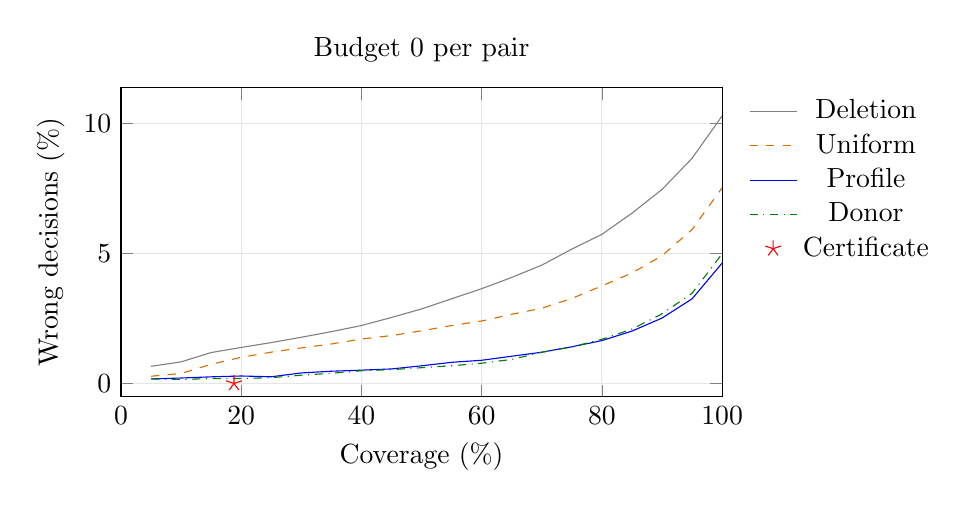
\begin{tikzpicture}
\begin{axis}[width=0.76\linewidth,height=5.5cm,tick label style={font=\normalsize},label style={font=\normalsize},legend style={font=\normalsize,draw=none},grid=major,grid style={gray!20},scaled ticks=false,xmin=0,xmax=100,ymin=-0.5,xlabel={Coverage (\%)},ylabel={Wrong decisions (\%)},legend pos=outer north east,title={Budget 0 per pair}]
\addplot+[gray,mark=none] coordinates {(5,0.6576670128) (10,0.8307372793) (15,1.18841583) (20,1.384562132) (25,1.57147802) (30,1.776854736) (35,1.992780497) (40,2.228279682) (45,2.538363909) (50,2.866043614) (55,3.256867743) (60,3.646013615) (65,4.079133051) (70,4.55174801) (75,5.16903196) (80,5.737279335) (85,6.550200558) (90,7.463174493) (95,8.662622288) (100,10.29421945)};
\addlegendentry{Deletion}
\addplot+[orange!85!black,mark=none,dashed] coordinates {(5,0.2769124264) (10,0.3807545864) (15,0.7384331372) (20,1.003807546) (25,1.204569055) (30,1.367255106) (35,1.518073481) (40,1.709068882) (45,1.842236837) (50,2.024922118) (55,2.22788634) (60,2.4027922) (65,2.659956866) (70,2.892745883) (75,3.269874236) (80,3.753461405) (85,4.249384073) (90,4.915195569) (95,5.920824908) (100,7.526825891)};
\addlegendentry{Uniform}
\addplot+[blue,mark=none] coordinates {(5,0.1730702665) (10,0.2076843198) (15,0.2538363909) (20,0.2855659398) (25,0.2561439945) (30,0.4038306219) (35,0.469762152) (40,0.5105572863) (45,0.5576708588) (50,0.6784354448) (55,0.8118568866) (60,0.8913118726) (65,1.046409458) (70,1.201602136) (75,1.409945771) (80,1.648494289) (85,2.013723454) (90,2.515287874) (95,3.255542803) (100,4.62962963)};
\addlegendentry{Profile}
\addplot+[green!50!black,mark=none,dashdotted] coordinates {(5,0.1730702665) (10,0.1557632399) (15,0.1846082843) (20,0.1903772932) (25,0.2215299412) (30,0.3172954886) (35,0.3906443159) (40,0.4889235029) (45,0.5307488174) (50,0.6057459328) (55,0.6796941376) (60,0.7788161994) (65,0.9239289613) (70,1.199129704) (75,1.403022961) (80,1.69825199) (85,2.091096044) (90,2.676820122) (95,3.470514292) (100,4.986154379)};
\addlegendentry{Donor}
\addplot+[red,only marks,mark=star,mark size=3pt] coordinates {(18.79196954,0)};
\addlegendentry{Certificate}
\end{axis}
\end{tikzpicture}

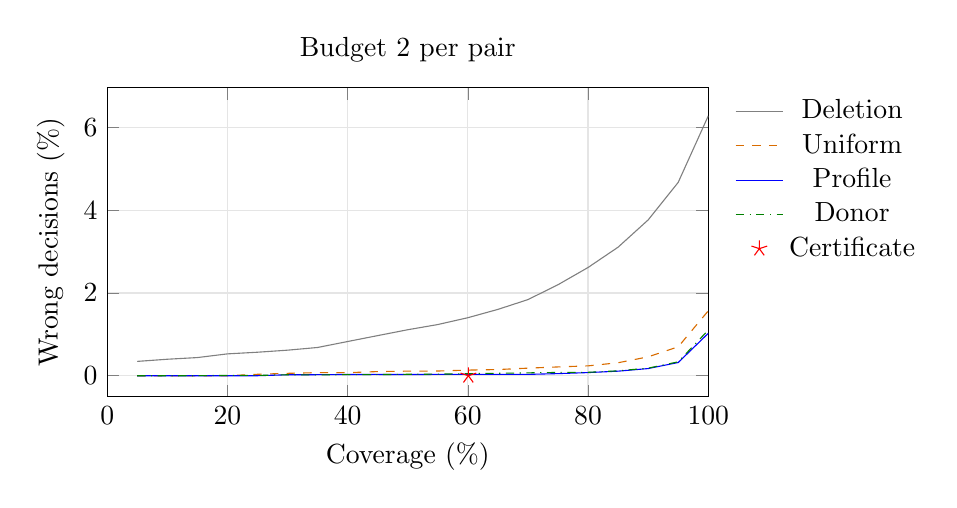
\begin{tikzpicture}
\begin{axis}[width=0.76\linewidth,height=5.5cm,tick label style={font=\normalsize},label style={font=\normalsize},legend style={font=\normalsize,draw=none},grid=major,grid style={gray!20},scaled ticks=false,xmin=0,xmax=100,ymin=-0.5,xlabel={Coverage (\%)},ylabel={Wrong decisions (\%)},legend pos=outer north east,title={Budget 2 per pair}]
\addplot+[gray,mark=none] coordinates {(5,0.3461405331) (10,0.398061613) (15,0.4384446752) (20,0.5278643129) (25,0.5676704742) (30,0.6172839506) (35,0.6823913366) (40,0.8264105227) (45,0.9691934926) (50,1.111111111) (55,1.236665723) (60,1.401869159) (65,1.60289693) (70,1.83948969) (75,2.199146187) (80,2.615524403) (85,3.107120314) (90,3.765239798) (95,4.672897196) (100,6.27898927)};
\addlegendentry{Deletion}
\addplot+[orange!85!black,mark=none,dashed] coordinates {(5,0) (10,0) (15,0) (20,0) (25,0.03461405331) (30,0.05769008884) (35,0.07417297137) (40,0.07355486327) (45,0.09999615399) (50,0.1107649706) (55,0.1132823563) (60,0.1355717088) (65,0.1491066912) (70,0.182959996) (75,0.2122995269) (80,0.2379716165) (85,0.3135626005) (90,0.4557517019) (95,0.697746443) (100,1.568016615)};
\addlegendentry{Uniform}
\addplot+[blue,mark=none] coordinates {(5,0) (10,0) (15,0) (20,0) (25,0) (30,0.02307603554) (35,0.02472432379) (40,0.03028729664) (45,0.03076804738) (50,0.02769124264) (55,0.03146732119) (60,0.03461405331) (65,0.03195143382) (70,0.03214162093) (75,0.05076727818) (80,0.07571824161) (85,0.1099505223) (90,0.1730702665) (95,0.3188136489) (100,1.024575978)};
\addlegendentry{Profile}
\addplot+[green!50!black,mark=none,dashdotted] coordinates {(5,0) (10,0) (15,0) (20,0.008653513326) (25,0.006922810661) (30,0.02307603554) (35,0.01977945903) (40,0.02596053998) (45,0.02692204146) (50,0.03461405331) (55,0.03776078542) (60,0.04903657552) (65,0.05857762867) (70,0.06922810661) (75,0.07845852083) (80,0.0822083766) (85,0.1180950054) (90,0.1826852813) (95,0.3352097794) (100,1.100726895)};
\addlegendentry{Donor}
\addplot+[red,only marks,mark=star,mark size=3pt] coordinates {(60.08653513,0)};
\addlegendentry{Certificate}
\end{axis}
\end{tikzpicture}

\caption{Frozen restricted-record daily evaluation; no saved-archive reconstruction. Daily error versus coverage in the Portugal panel, six-hour gaps and exact six-hour totals. Every evaluator receives the same optimal-batch recovered values at budget two. Curves select by visible estimated margins; the star shows the sharp method\textquotesingle s attained coverage and observed error. Complete-reference losses are used only after selection to count errors. All values are descriptive on this fixed panel.}
\label{fig:dailycoverage}\end{figure}
\FloatBarrier

\subsection{Named competitors and comparison difficulty}\label{app:named-pairs}
Table~\ref{tab:namedpairs} separates every model pair in the primary panel,
including ridge versus boosting and ridge versus MLP. These comparisons
prevent aggregate coverage from being attributed solely to the difference
between persistence and learned forecasts. The complete-reference margin
strata in Table~\ref{tab:marginstrata} further isolate close daily comparisons;
they are explanatory strata formed after evaluation, not information
available to the audit.
\begin{table}[htbp]
\centering\normalsize\setlength{\tabcolsep}{4pt}
\caption{Frozen restricted-record daily evaluation; no saved-archive reconstruction. Certified daily comparisons (\%) by named model pair, six-hour gaps and exact six-hour totals. The full cohort and pair breakdown is in \texttt{study\_daily\_pairs.csv}.}
\label{tab:namedpairs}
\begin{tabular}{lrr}
\toprule
Portugal model pair & Before & Budget two\\
\midrule
Daily--Boosting & 24.9 & 66.2\\
Daily--MLP & 21.5 & 61.7\\
Daily--Ridge & 25.5 & 67.1\\
Boosting--MLP & 10.7 & 51.3\\
Ridge--Boosting & 16.5 & 59.4\\
Ridge--MLP & 13.7 & 54.8\\
\bottomrule
\end{tabular}
\end{table}
\begin{table}[htbp]
\centering\normalsize\setlength{\tabcolsep}{4pt}
\caption{Frozen restricted-record daily evaluation; no saved-archive reconstruction. Portugal certification (\%) by increasing absolute normalized complete-reference daily loss margin, pooled over all six pairs. Quintile 1 contains the closest comparisons. The same cases define each stratum at both budgets; repeated mask seeds remain dependent. Pair-specific strata are archived in \texttt{study\_daily\_margin\_strata.csv}.}
\label{tab:marginstrata}
\begin{tabular}{lrrrr}
\toprule
Quintile & Min. margin & Max. margin & Before & Budget two\\
\midrule
1 & $2.853\times10^{-7}$ & 0.0014627 & 0.1 & 11.2\\
2 & 0.0014628 & 0.003581 & 1.0 & 40.2\\
3 & 0.0035814 & 0.0081389 & 6.3 & 66.0\\
4 & 0.0081464 & 0.021704 & 21.9 & 85.5\\
5 & 0.021704 & 4.0102 & 64.7 & 97.6\\
\bottomrule
\end{tabular}
\end{table}
In the closest-margin quintile, budget-two certification is
11.17\%, versus
97.56\% in the widest-margin quintile.
Recovery therefore helps close comparisons but does not remove their
identification difficulty. The named learned-model comparisons and the
small-margin strata should be considered together when assessing a use case.
\FloatBarrier


\subsection{Comparisons involving the neural forecaster}\label{app:neural-pairs}
Table~\ref{tab:neural} isolates MLP-versus-persistence, MLP-versus-ridge,
and MLP-versus-boosting comparisons, keeping every meter, test day, and
mask seed. This prevents the AI conclusion from resting only on an
aggregate that includes comparisons between simpler models. The audit
requires saved predictions and measurement constraints, so its procedure
is identical for the neural and other candidates. These results establish
its applicability to the trained MLP; they do not establish a new neural
architecture or state-of-the-art forecasting accuracy.
\begin{table*}[htbp]
\centering\normalsize\setlength{\tabcolsep}{4pt}
\caption{Frozen restricted-record daily evaluation; no saved-archive reconstruction. AI-specific audit: resolution (\%) for the three comparisons involving the neural MLP, six-hour gaps and exact six-hour totals. Before: no recovery. All other columns use budget two. This subset was specified before the revised results were calculated.}
\label{tab:neural}
\begin{tabular}{lrrrrrrr}
\toprule
Source & Before & Optimal & Greedy & Uniform random & Max. $|c|$ & Wt. $|c|$ & Wt. $c^2$\\
\midrule
Portugal & 15.3 & 55.9 & 54.8 & 32.5 & 43.0 & 35.4 & 38.0\\
Household & 44.4 & 87.8 & 86.5 & 68.2 & 78.5 & 72.5 & 75.4\\
Counters & 39.8 & 86.2 & 85.5 & 64.8 & 78.1 & 70.7 & 74.3\\
\bottomrule
\end{tabular}
\end{table*}
Figure~\ref{fig:recovery} displays coverage and worst-case width across budgets.
\begin{figure}[htbp]\centering
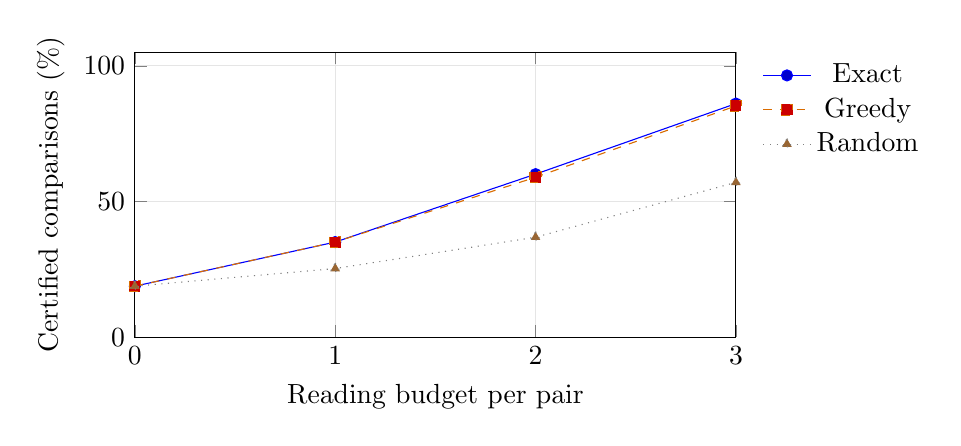
\begin{tikzpicture}
\begin{axis}[width=0.76\linewidth,height=5.2cm,tick label style={font=\normalsize},label style={font=\normalsize},legend style={font=\normalsize,draw=none},grid=major,grid style={gray!20},scaled ticks=false,xmin=0,xmax=3,xtick={0,1,2,3},ymin=0,ymax=105,xlabel={Reading budget per pair},ylabel={Certified comparisons (\%)},legend pos=outer north east]
\addplot+[blue,mark=*] coordinates {(0,18.79196954) (1,35.05019038) (2,60.08653513) (3,86.07995846)};
\addlegendentry{Exact}
\addplot+[orange!85!black,mark=square*,dashed] coordinates {(0,18.79196954) (1,35.05019038) (2,58.93388716) (3,85.22499135)};
\addlegendentry{Greedy}
\addplot+[gray,mark=triangle*,dotted] coordinates {(0,18.79196954) (1,25.29075805) (2,36.84146764) (3,57.04742125)};
\addlegendentry{Random}
\end{axis}
\end{tikzpicture}

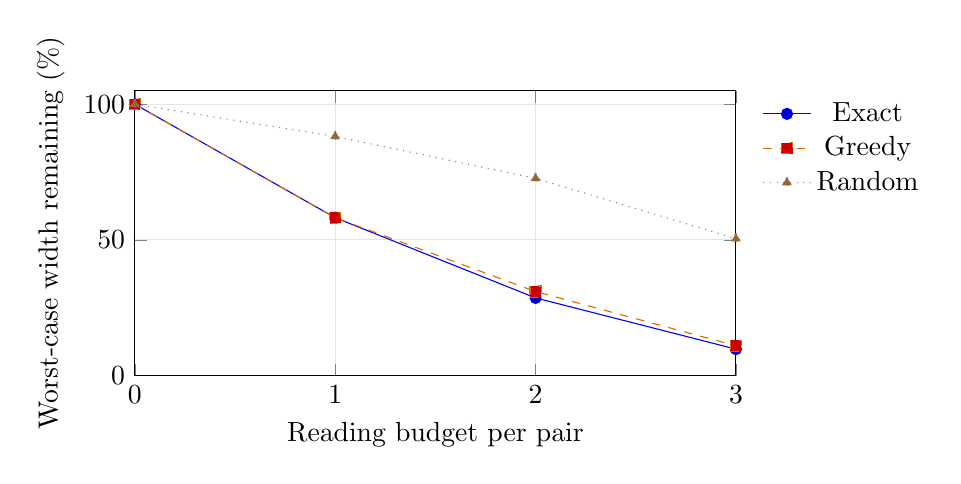
\begin{tikzpicture}
\begin{axis}[width=0.76\linewidth,height=5.2cm,tick label style={font=\normalsize},label style={font=\normalsize},legend style={font=\normalsize,draw=none},grid=major,grid style={gray!20},scaled ticks=false,xmin=0,xmax=3,xtick={0,1,2,3},ymin=0,ymax=105,xlabel={Reading budget per pair},ylabel={Worst-case width remaining (\%)},legend pos=outer north east]
\addplot+[blue,mark=*] coordinates {(0,100) (1,58.18690041) (2,28.62983522) (3,9.755222493)};
\addlegendentry{Exact}
\addplot+[orange!85!black,mark=square*,dashed] coordinates {(0,100) (1,58.18690041) (2,30.97520219) (3,11.00077593)};
\addlegendentry{Greedy}
\addplot+[gray,mark=triangle*,dotted] coordinates {(0,100) (1,88.13802378) (2,72.69957825) (3,50.45326371)};
\addlegendentry{Random}
\end{axis}
\end{tikzpicture}

\caption{Frozen restricted-record daily evaluation; no saved-archive reconstruction. Recovery in the Portugal panel: six missing hourly targets, exact six-hour totals, all six model pairs and three mask seeds. Curves are means of per-meter results. Top: realized certification coverage. Bottom: worst-case width relative to its no-recovery value, the criterion optimized. A width advantage need not give a coverage advantage at the observed truth.}
\label{fig:recovery}\end{figure}
\FloatBarrier

\subsection{Incremental benefit over greedy retrieval}\label{app:greedy-detail}
The gain over no recovery combines acquiring new data with selecting them.
To isolate allocation, we compare exact and greedy selection at the same
budget on every case. In Portugal at six missing hours and budget two,
the mean meter-level resolution difference is 1.15 percentage
points, with meter-level range 0.21 to 2.49.
The median is 1.19; across meter--seed summaries
the 10th and 90th percentiles are 0.47 and 1.87 points.
Exact selection alone resolves 785 dependent cases,
whereas greedy alone resolves 119. Thus the worst-case-width
optimum is not a pointwise optimum for realized certification.

Across these cases, the additional worst-case-width reduction of exact
over greedy, divided by initial width, has median 0.00\%, 90th percentile
3.41\%, and maximum 92.02\%.
Realized width is larger under the exact policy in 700 cases;
that outcome is compatible with optimizing a worst-case objective.
The complete signed distributions and pair/seed breakdowns are retained in
\texttt{recovery\_diagnostics.json}, \texttt{study\_recovery\_pair\_seed.csv},
and the full local \texttt{study\_recovery\_cases.csv}. The public package
supplies \texttt{study\_recovery\_cases\_public.csv} for UCI cases and
hashes plus regeneration instructions for the omitted BLEM case rows.
These post-review diagnostics include
all cases and are descriptive; repeated days, pairs, and seeds are dependent.
Table~\ref{tab:actualrecovery} complements the budget caps with actual query
counts and both realized and worst-case remaining widths.
\begin{table*}[htbp]
\centering\normalsize\setlength{\tabcolsep}{4pt}
\caption{Frozen restricted-record daily evaluation; no saved-archive reconstruction. Actual mean reading counts and remaining-width fractions (\%) at budget two, six-hour gaps and totals. Within-meter width fractions divide summed remaining width by summed initial width; cohort values macro-average meters. Queries are per specified pair, not the cost of ranking all four models. All policies and budgets appear in \texttt{study\_recovery.csv}.}
\label{tab:actualrecovery}
\begin{tabular}{llrrrr}
\toprule
Source & Policy & Queries & Actual width & Worst width & Resolved\\
\midrule
Portugal & Exact & 1.999 & 19.1 & 28.6 & 60.1\\
Portugal & Greedy & 1.999 & 20.5 & 31.0 & 58.9\\
Portugal & Uniform random & 1.999 & 47.8 & 72.7 & 36.8\\
Household & Exact & 2.000 & 17.2 & 25.7 & 89.2\\
Household & Greedy & 2.000 & 18.7 & 28.1 & 88.3\\
Household & Uniform random & 2.000 & 48.4 & 71.4 & 71.1\\
Counters & Exact & 2.000 & 15.6 & 23.5 & 86.9\\
Counters & Greedy & 2.000 & 16.7 & 25.3 & 86.2\\
Counters & Uniform random & 2.000 & 46.5 & 69.2 & 67.3\\
\bottomrule
\end{tabular}
\end{table*}
Table~\ref{tab:recoveryci} summarizes the paired meter-bootstrap
stability of the resolution gains, separately for all pairs and neural-model
pairs. Whole meters remain the resampling unit.
\begin{table}[htbp]
\centering\normalsize\setlength{\tabcolsep}{4pt}
\caption{Frozen restricted-record daily evaluation; no saved-archive reconstruction. Portugal resolution gain in percentage points: optimal recovery with budget two minus the reference policy, six-hour gaps and exact six-hour totals. Lower/Upper: descriptive 95\% paired bootstrap limits from 2,000 resamples of the same 30 whole meters. All days, pairs, and seeds remain aggregated within each meter. These are panel-stability intervals, not population-wide confidence claims.}
\label{tab:recoveryci}
\begin{tabular}{llrrr}
\toprule
Comparisons & Reference & Gain & Lower & Upper\\
\midrule
All pairs & No recovery & 41.29 & 38.85 & 43.52\\
All pairs & Greedy & 1.15 & 1.01 & 1.31\\
All pairs & Weighted $|c|$ & 19.83 & 18.58 & 20.87\\
All pairs & Weighted $c^2$ & 16.98 & 15.90 & 17.91\\
MLP pairs & No recovery & 40.64 & 38.67 & 42.69\\
MLP pairs & Greedy & 1.18 & 0.99 & 1.36\\
MLP pairs & Weighted $|c|$ & 20.56 & 19.40 & 21.56\\
MLP pairs & Weighted $c^2$ & 17.89 & 16.82 & 18.77\\
\bottomrule
\end{tabular}
\end{table}
\FloatBarrier

\subsection{Sensitivity to the available forecast archive}\label{app:earlier-access}\label{sec:archive-access}
Allowing the saved future persistence forecasts changes the information
problem substantially (Table~\ref{tab:archive-access}). The lookup reveals
most masked targets without paid recovery. These results are not additional
improvements attributable to the query optimizer: they arise from using
information already present in the broader archive.

\begin{table}[htbp]
\centering\small
\caption{Access to all available saved test persistence forecasts. Free:
percentage of originally masked target occurrences revealed before queries.
$C_0,C_2$: certified comparison percentages at zero and at most two paid
queries using the exact policy. $\Delta$: exact-minus-greedy $C_2$ in
percentage points. $\bar q$: actual mean paid queries per pair at budget two.
All figures include every case, not only previously unresolved comparisons.}
\label{tab:archive-access}
\begin{tabular}{lrrrrrr}
\toprule
Cohort & Gap (h) & Free (\%) & $C_0$ & $C_2$ & $\Delta$ & $\bar q$\\
\midrule
Portugal & 6 & 95.33 & 96.67 & 98.71 & +0.042 & 0.093\\
Portugal & 12 & 95.33 & 95.70 & 96.17 & +0.014 & 0.093\\
Household & 6 & 88.21 & 93.50 & 98.71 & +0.226 & 0.236\\
Household & 12 & 88.21 & 89.79 & 92.86 & +0.090 & 0.236\\
Counters & 6 & 98.90 & 99.45 & 99.82 & +0.020 & 0.022\\
Counters & 12 & 98.90 & 98.96 & 99.25 & +0.000 & 0.022\\
\bottomrule
\end{tabular}
\end{table}
The saved persistence copies match the reference targets exactly in the
stored binary64 data. Every recomputed comparison interval contains its
reference difference, and no certificate is incorrect. The restricted
regime reproduces 5,168
archived meter and named-pair/seed rows, including decision counts,
widths and mean queries. The sensitivity evaluates 1,073,952
dependent policy/budget/pair cases; this is a computation count, not an
independent statistical sample.

The large restricted-record gain from paid recovery therefore does not
carry over unchanged to an archive with these future exact copies.
The remaining uncertainty is concentrated at boundaries and gaps in the
available test archive. A practical audit should incorporate authorized
reconstructable targets first and allocate a recovery budget only to the
remaining unknowns. This analysis supports that workflow, but does not
measure field retrieval savings or establish how often a real evaluator
has only the restricted inputs.

\FloatBarrier

\subsection{Replication on 30 previously unused consumers}\label{app:replication-results}
\label{sec:newconsumers}
Table~\ref{tab:newconsumers} reports the replication. The fixed training-only rule selected 30 additional consumers from 255
eligible candidates. Each contributes 107 test days, giving 3,210
additional meter-days and 77,040 hourly targets.
The supplied targets and fixed forecasts range from 0.00 to
3,440.43 kWh per hourly target.
All 30 neural fits stopped in 28--383 epochs within the fixed allowance, with no captured training warnings. The analysis retains all 57,780
pair/mask comparisons per access regime. Policy and budget evaluations of
the same records are dependent; they are not additional independent samples.

\begin{table}[t]
\centering\small
\caption{Daily outcomes over three mask seeds. Frozen new-consumer replication: mean consumer-level certification
rates (\%) under six-hour gaps and totals. $q\leq2$ denotes an available
two-reading budget per model pair. Final column: mean readings actually
queried by exact recovery.}
\label{tab:newconsumers}
\begin{tabular}{lrrrr}
\toprule
Access & $q=0$ & Exact $q\leq2$ & Greedy $q\leq2$ & Queries\\
\midrule
Restricted record & 25.02 & 64.11 & 62.95 & 1.998\\
Saved archive & 96.87 & 98.57 & 98.51 & 0.093\\
\bottomrule
\end{tabular}
\end{table}

Restricted-record exact-minus-greedy coverage is 1.154 percentage points (descriptive 95\% consumer-bootstrap interval [1.004, 1.303]); 30 consumers favor exact recovery, 0 favor greedy and 0 tie.
Saved-archive exact-minus-greedy coverage is 0.061 percentage points (descriptive 95\% consumer-bootstrap interval [0.035, 0.088]); 18 consumers favor exact recovery, 2 favor greedy and 10 tie.
The saved archive reconstructs 95.327\% of masked targets without a query. No incorrect certificate,
truth-enclosure failure or violation of the predicted worst remaining
width occurred in the 462,240 dependent policy/budget
evaluations. Query eligibility and copied target values also passed the
recorded checks. Per-consumer, named-pair, seed and forecast-error tables,
along with these UCI-only predictions, are supplied for reconstruction.
This replication tests the fixed procedure beyond its development panel;
it does not supply production outage, target-arrival or retrieval-cost data.

A separate checker, importing none of the analysis implementations,
recomputes all 120 forecast-error rows and
115,560 zero-query comparisons,
and reconciles all pair/seed, consumer, cohort and named-pair aggregates.
Representative numerical checks additionally enumerate 2,882 direct-loss vertices
and 5,994 query subsets.
This is a separate implementation within the same study; it does not
independently refit the forecasts or reproduce every two-query case.
\FloatBarrier

\subsection{Recovery with interval totals on real traces}\label{app:interval-results}
\label{sec:interval-trace-recovery}
Table~\ref{tab:interval-trace-recovery} reports every cohort, access regime
and total-uncertainty setting. Under restricted daily access, widening the
Portugal totals from exact values to $\pm5\%$ lowers two-query certification
from 60.1\% to 46.3\%.
Recovery still increases certification from 15.8\%
at zero queries. With saved-archive access and $\pm5\%$ totals, the change
is smaller: 96.5\% to 98.1\%.
The exact-minus-greedy certification differences at this setting are
1.163 and
0.050 percentage points,
respectively. The corresponding reductions in mean realized width,
normalized by squared training mean energy, are
0.001249 and
0.000071.
These are observed increments, not approximation guarantees for certification.

\begin{table*}[htbp]
\centering\normalsize\setlength{\tabcolsep}{4pt}
\caption{Recovery under constructed total intervals on real traces. $\tau$: total half-width (\%). D: isolated daily record with exact deductions; A: all saved persistence copies plus exact deductions. $C_0$: certification without paid queries; $C_E,C_G$: certification after at most two queries per day/pair for exact and greedy batches (\%). $W_E,W_G$: remaining worst width as a percentage of initial width, computed as a within-meter ratio of sums and then macro-averaged. Zero initial width contributes zero to this ratio. All observed certificates were correct; repeats are dependent.}
\label{tab:interval-trace-recovery}
\begin{tabular}{lrlrrrrr}
\toprule
Source & $\tau$ & Access & $C_0$ & $C_E$ & $C_G$ & $W_E$ & $W_G$\\
\midrule
Portugal & 0 & D & 18.8 & 60.1 & 58.9 & 28.6 & 31.0\\
Portugal & 1 & D & 18.1 & 56.8 & 55.7 & 30.2 & 32.5\\
Portugal & 5 & D & 15.8 & 46.3 & 45.2 & 35.1 & 37.4\\
Portugal & 0 & A & 96.7 & 98.7 & 98.7 & 27.4 & 30.3\\
Portugal & 1 & A & 96.6 & 98.6 & 98.5 & 29.3 & 32.1\\
Portugal & 5 & A & 96.5 & 98.1 & 98.0 & 35.2 & 37.9\\
Household & 0 & D & 48.9 & 89.2 & 88.3 & 25.7 & 28.1\\
Household & 1 & D & 47.9 & 88.1 & 87.1 & 26.8 & 29.2\\
Household & 5 & D & 44.6 & 83.9 & 82.7 & 30.6 & 33.1\\
Household & 0 & A & 93.5 & 98.7 & 98.5 & 24.5 & 26.0\\
Household & 1 & A & 93.4 & 98.6 & 98.4 & 25.7 & 27.2\\
Household & 5 & A & 93.0 & 98.2 & 98.1 & 29.8 & 31.6\\
Counters & 0 & D & 43.9 & 86.9 & 86.2 & 23.5 & 25.3\\
Counters & 1 & D & 42.9 & 85.8 & 85.1 & 24.6 & 26.4\\
Counters & 5 & D & 39.8 & 81.7 & 80.6 & 28.1 & 30.0\\
Counters & 0 & A & 99.5 & 99.8 & 99.8 & 15.3 & 16.4\\
Counters & 1 & A & 99.5 & 99.8 & 99.8 & 16.0 & 17.0\\
Counters & 5 & A & 99.4 & 99.8 & 99.8 & 18.4 & 19.3\\
\bottomrule
\end{tabular}
\end{table*}

No incorrect certificate, truth-enclosure failure, or realized-width
violation occurred in 1,610,928
dependent policy/budget evaluations. Exact worst width never exceeded
greedy worst width in the 402,732
matched cases. At zero total uncertainty,
134,244 initial-bound
and optimal-objective comparisons agree with the original exact-total
implementation within the declared numerical tolerance;
all 268,488 compared query
tuples and their decisions are unchanged. The largest discrepancy in the
reconciled cohort mean worst width is \texttt{2.84e-14}.
Independent integration fixtures additionally verify
192
linear-program endpoints, with maximum absolute discrepancy
\texttt{1.33e-15}; these floating-point checks
do not provide outward-rounded enclosures. Source hashes confirm that the
original archives and implementations are unchanged.
A separate aggregation script reconstructs all meter, cohort and policy
comparison tables from the saved pair/seed summaries; it does not rerun
the raw-trace experiment.
The sensitivity demonstrates behavior under specified total intervals on
real load shapes. It does not estimate physical meter-error distributions,
retrieval cost, response latency, or operational savings.




\FloatBarrier
\section{Conservative Selection When Ordering Is Unresolved}\label{app:regret}
Let $U_{jk}=\max_{y\in\F}(L_j(y)-L_k(y))$, with $U_{jj}=0$.
For a finite set of fixed candidates define
\begin{equation}
 R_j=\max_{y\in\F}\{L_j(y)-\min_k L_k(y)\}.
 \label{eq:regret}
\end{equation}
The comparator is the best member of this candidate set for the completed
record. It is not a forecast that had advance access to the targets.
\begin{proposition}[Regret from pairwise bounds]
For a common nonempty compact feasible set,
\begin{equation}
 R_j=\max_k U_{jk},\qquad
 j^*\in\arg\min_j\max_k U_{jk}.
 \label{eq:minimax}
\end{equation}
Consequently, $j^*$ minimizes the worst-case empirical regret among the
available candidates.
\end{proposition}
\begin{proof}
$L_j(y)-\min_kL_k(y)=\max_k(L_j(y)-L_k(y))$.
Taking a maximum over $y$ commutes with the finite maximum over $k$.
Both sides optimize over the same product of the feasible set and candidate
index set. No interchange of a minimum and a maximum is required.
\end{proof}
For every $y\in\F$, the selected candidate's realized regret is at most
$R_{j^*}$. This guarantee is conditional on the measurement constraints
containing the relevant truth. It does not imply that the minimax choice
has the smallest regret at every particular completion. An imputation-based
choice can perform better at the actual reference record; both realized
regret and the worst-case bound are therefore evaluated.


\subsection{Observed selection tradeoff}
Table~\ref{tab:regret} retains realized regret and the exact worst-case
criterion for every evaluated selector in the six-hour-gap/six-hour-total
setting. A small worst-case bound is a different objective from a small
regret at the actual reference completion. This extension should be used
only when that conservative criterion is relevant; it does not establish
that minimax selection improves average prediction accuracy.
\begin{table*}[htbp]
\centering\normalsize\setlength{\tabcolsep}{4pt}
\caption{Frozen restricted-record daily evaluation; no saved-archive reconstruction. Selection tradeoff for contiguous six-target gaps and exact six-hour totals. Entries are $10^3$ times normalized realized regret and worst-case regret bound. Tail actual is the mean of individual meters\textquotesingle\ 95th-percentile regrets, not a pooled percentile. Every realized regret was within its corresponding bound. Minimax reduces the worst-case criterion but does not minimize observed regret.}
\label{tab:regret}
\begin{tabular}{llrrr}
\toprule
Source & Selector & Mean actual & Tail actual & Mean bound\\
\midrule
Portugal & Deletion & 1.123 & 5.238 & 34.126\\
Portugal & Uniform & 0.433 & 2.416 & 32.262\\
Portugal & Profile & 0.198 & 1.085 & 32.492\\
Portugal & Donor & 0.195 & 0.896 & 32.731\\
Portugal & Minimax regret & 1.549 & 7.382 & 27.283\\
Household & Deletion & 9.540 & 59.321 & 117.518\\
Household & Uniform & 1.443 & 8.484 & 103.739\\
Household & Profile & 1.106 & 4.018 & 105.996\\
Household & Donor & 2.664 & 14.220 & 111.310\\
Household & Minimax regret & 6.809 & 48.240 & 93.646\\
Counters & Deletion & 19.132 & 100.609 & 175.961\\
Counters & Uniform & 5.106 & 29.035 & 153.845\\
Counters & Profile & 2.556 & 14.072 & 153.035\\
Counters & Donor & 3.655 & 19.691 & 157.434\\
Counters & Minimax regret & 11.114 & 64.649 & 137.404\\
\bottomrule
\end{tabular}
\end{table*}



\FloatBarrier
\section*{Supplementary Materials}
\textbf{Online Resource 1: Reproducibility package.}
The accompanying \texttt{research\_supplement.zip} contains implementations,
source-download and reproduction scripts, dated protocols, aggregate
results, frozen fitted-model forecasts, validation reports, and the
manuscript reconstruction scripts.

\section*{Statements and Declarations}
\subsection*{Data and Code Availability}
The source datasets are publicly identified in References
\cite{uci,portugal,blem}. Reproduction code, the documented protocol and its
dated amendments, complete scenario summaries, and
validation results accompany this manuscript as supplementary materials.
The supplement identifies exact source versions and checksums and recreates
the hourly targets from the original sources. The original fitting pipeline
is supplied separately from the no-refit evaluation reproduction.
\texttt{frozen\_forecasts.csv} supplies saved fitted-model forecasts for all
34 series, target timestamps, and simulated issue-time cutoffs; it also
includes persistence for the two UCI sources. BLEM persistence is omitted
because it directly copies earlier raw readings and can be regenerated.
For exact reproduction, \texttt{review\_frozen\_forecasts.csv} preserves
the original fitted-forecast text and the UCI targets, with only BLEM
targets and persistence omitted. Combining this lossless export with the
pinned raw targets restores all 89,496 original evaluation rows to the
original byte-level SHA-256 checksum without refitting. That reconstruction
has been executed; the supplied \texttt{--raw} mode reruns the corrected
analyses from these restored records. The default
\texttt{work/reproduce\_review\_revision.py} command independently checks
distributed UCI period traces and interval aggregates and rebuilds the
manuscript. Its BLEM checks reconcile aggregates; detailed BLEM case
reconstruction requires the full local records or raw mode. Full period
traces, archive-aware case endpoints and old per-day recovery cases that
could reveal omitted BLEM readings are replaced by UCI-only public exports
and omission manifests. Full local and raw-mode period checks cover all
34 series. The default mode does not claim an independent forecast refit
or a raw-data rerun.
The separate UCI-only new-consumer replication supplies its hourly targets
and all four forecasts under the source's CC BY 4.0 terms, with attribution
and preprocessing documented in the supplement.
The full
per-hour prediction/target archive is retained for the local analysis but
omitted from the submission supplement because a separate redistribution
license for the BLEM readings was not verified. Its checksum is recorded
so regenerated files can be checked. No public
repository publication is claimed beyond the cited original data sources.


The additional randomized-recovery materials include the compact optimizer,
an executable hard-budget sampler, complete finite-game primal/dual traces,
all positive query batches, an independent reconstruction of every public
energy case, and sharpness/scalability fixtures. The NOAA materials include
the selected observation records, decoded gridpoint predictions and message
provenance, the fixed source-selection protocol, all nine natural cases,
all 43 dry controls, failed-run diagnostics and the declared preprocessing
and tolerance sensitivities. Source URLs and content hashes identify the
downloaded records; the supplement does not include the large GRIB cache.
The naturally missing subdaily targets are not available as reference truth.

\subsection*{Research Transparency}
This study reanalyzes public meter and precipitation records and does not recruit participants
or collect new measurements. Artificial outages, constructed totals,
recorded counter increments, and assumed total-error ranges are distinguished
in the methods. All reported numerical results were calculated by the
accompanying code.

\subsection*{Funding and Competing Interests}
\textbf{Funding.} This research received no external funding.

\textbf{Competing interests.} The author declares no conflicts of interest.

\subsection*{Generative-AI Disclosure}
OpenAI Codex (OpenAI; accessed October 2026) assisted with literature
searches, mathematical review, programming, experimental execution, and
manuscript drafting. This assistance is distinct from the trained MLP and
boosted-tree forecasting models evaluated in the study.

\FloatBarrier
\begin{thebibliography}{99}

\bibitem{azuremonitor} Microsoft, ``Monitor the performance of models deployed
to production,'' Azure Machine Learning documentation, updated 11 February
2026. \url{https://learn.microsoft.com/en-us/azure/machine-learning/how-to-monitor-model-performance?view=azureml-api-2}.
\bibitem{awsmonitor} Amazon Web Services, ``Model Monitor FAQs,'' Amazon
SageMaker AI Developer Guide, accessed 9 October 2026.
\url{https://docs.aws.amazon.com/sagemaker/latest/dg/model-monitor-faqs.html}.
\bibitem{canada} Measurement Canada, ``GEN-31---Policy on multirate register
metering,'' sec.~5.7, revised 2010.
\url{https://ised-isde.canada.ca/site/measurement-canada/en/laws-and-requirements/gen-31-policy-multirate-register-metering}.
\bibitem{norpen} A. Vavouris, F. Guasselli, L. Stankovic, V. Stankovic,
K. Gram-Hanssen, and S. Didierjean, ``Descriptor: A Norwegian positive
energy neighborhood dataset of electrical measurements and interviews on
energy practices (NorPEN),'' \emph{IEEE Data Descriptions}, vol.~1, 2024.
\url{https://doi.org/10.1109/IEEEDATA.2024.3483154}.
\bibitem{elexon} Elexon, ``BSCP702: Advanced Data Service,'' version 2.0,
effective 6 November 2025, secs.~4.2.7A--B, 4.2.16--17, and 4.2.21.
\url{https://bscdocs.elexon.co.uk/bsc-module/bsc-procedures/bscp702-advanced-data-service}.
\bibitem{aemo} Australian Energy Market Operator,
``Metrology procedure: Part B---Metering data validation, substitution
and estimation,'' version~8.13, effective June~9, 2026,
secs.~2.4--2.5 and 3.2.
\url{https://www.aemo.com.au/-/media/files/electricity/nem/retail_and_metering/market_settlement_and_transfer_solutions/2026/metrology-procedure-part-b-v813-clean.pdf}.
\bibitem{manski} C. F. Manski, ``Partial identification with missing data:
Concepts and findings,'' \emph{International Journal of Approximate
Reasoning}, vol.~39, pp.~151--165, 2005.
\url{https://doi.org/10.1016/j.ijar.2004.10.006}.
\bibitem{polo} F. Maia Polo, S. Maity, M. Yurochkin, M. Banerjee, and
Y. Sun, ``Weak supervision performance evaluation via partial
identification,'' \emph{Advances in Neural Information Processing
Systems}, vol.~37, 2024. \url{https://arxiv.org/abs/2312.04601}.
\bibitem{bessac} J. Bessac and P. Naveau, ``Forecast score distributions
with imperfect observations,'' \emph{Advances in Statistical Climatology,
Meteorology and Oceanography}, vol.~7, pp.~53--71, 2021.
\url{https://doi.org/10.5194/ascmo-7-53-2021}.
\bibitem{botacin2025} M. Botacin and H. Gomes, ``Towards more realistic
evaluations: The impact of label delays in malware detection pipelines,''
\emph{Computers \& Security}, vol.~148, art.~104122, 2025.
\url{https://doi.org/10.1016/j.cose.2024.104122}.
\bibitem{patton} A. J. Patton, ``Volatility forecast comparison using
imperfect volatility proxies,'' \emph{Journal of Econometrics}, vol.~160,
no.~1, pp.~246--256, 2011. \url{https://doi.org/10.1016/j.jeconom.2010.03.034}.
\bibitem{cpi} M. Weber, M. Turowski, H. K. \c{C}akmak, R. Mikut,
U. K\"uhnapfel, and V. Hagenmeyer, ``Data-driven copy-paste imputation
for energy time series,'' \emph{IEEE Transactions on Smart Grid},
vol.~12, no.~6, pp.~5409--5419, 2021.
\url{https://doi.org/10.1109/TSG.2021.3101831}.
\bibitem{hu} S. Hu, H. Dai, F. Meng, L. Aslett, M. Pollock, and
G. O. Roberts, ``Statistical disaggregation---A Monte Carlo approach
for imputation under constraints,'' \emph{Scandinavian Journal of
Statistics}, vol.~52, no.~3, pp.~1376--1421, 2025.
\url{https://doi.org/10.1111/sjos.12790}.
\bibitem{heat} M. Schaffer, T. Tvedebrink, and A. Marszal-Pomianowska,
``Three years of hourly data from 3021 smart heat meters installed in
Danish residential buildings,'' \emph{Scientific Data}, vol.~9,
art.~420, 2022. \url{https://doi.org/10.1038/s41597-022-01502-3}.
\bibitem{savage} L. J. Savage, ``The theory of statistical decision,''
\emph{Journal of the American Statistical Association}, vol.~46,
pp.~55--67, 1951. \url{https://doi.org/10.1080/01621459.1951.10500768}.
\bibitem{manskiregret} C. F. Manski, ``Minimax-regret treatment choice
with missing outcome data,'' \emph{Journal of Econometrics}, vol.~139,
pp.~105--115, 2007. \url{https://doi.org/10.1016/j.jeconom.2006.06.006}.
\bibitem{sawade} C. Sawade, N. Landwehr, and T. Scheffer,
``Active comparison of prediction models,''
\emph{Advances in Neural Information Processing Systems}, vol.~25, 2012.
\url{https://proceedings.neurips.cc/paper_files/paper/2012/file/92fb0c6d1758261f10d052e6e2c1123c-Paper.pdf}.
\bibitem{hara} S. Hara, M. Matsuura, J. Honda, and S. Ito,
``Active model selection: A variance minimization approach,''
\emph{Machine Learning}, vol.~113, pp.~8327--8345, 2024.
\url{https://doi.org/10.1007/s10994-024-06603-1}.
\bibitem{active} J. Kossen, S. Farquhar, Y. Gal, and
T. Rainforth, ``Active testing: Sample-efficient model evaluation,''
\emph{Proceedings of Machine Learning Research}, vol.~139,
pp.~5753--5763, 2021.
\url{https://proceedings.mlr.press/v139/kossen21a.html}.
\bibitem{sensorsel} Y. Wang, M. Sznaier, and F. Dabbene,
``A convex optimization approach to worst-case optimal sensor selection,''
in \emph{Proceedings of the 52nd IEEE Conference on Decision and Control},
pp.~6353--6358, 2013.
\url{https://robustsystems.coe.neu.edu/sites/robustsystems.coe.neu.edu/files/systems/papers/Yin_CDC13.pdf}.
\bibitem{ddid} P. Vayanos, A. Georghiou, and H. Yu,
``Robust optimization with decision-dependent information discovery,''
\emph{Management Science}, vol.~72, no.~2, pp.~1509--1528, 2026
(published online June 2025).
\url{https://doi.org/10.1287/mnsc.2021.00160}.
\bibitem{aggarwal} A. Aggarwal, H. Imai, N. Katoh, and S. Suri, ``Finding
$k$ points with minimum diameter and related problems,'' \emph{Journal of
Algorithms}, vol.~12, no.~1, pp.~38--56, 1991,
\url{https://doi.org/10.1016/0196-6774(91)90022-Q}.
\bibitem{chen2026} X. Chen, M. Goerigk, and M. Poss, ``The robust selection
problem with information discovery,'' \emph{Discrete Applied Mathematics},
vol.~382, pp.~277--292, 2026. \url{https://doi.org/10.1016/j.dam.2025.12.012}.
\bibitem{iancu2014} D. A. Iancu and N. Trichakis, ``Pareto efficiency in robust
optimization,'' \emph{Management Science}, vol.~60, no.~1, pp.~130--147, 2014.
\url{https://doi.org/10.1287/mnsc.2013.1753}.

% Verified against the official Springer article/chapter pages, 10 October 2026.
% Kawase--Sumita appeared online in 2023; its journal volume year is 2024.
\bibitem{kawase2024}
Y.~Kawase and H.~Sumita, ``Randomized strategies for robust combinatorial
optimization with approximate separation,'' \emph{Algorithmica}, vol.~86,
pp.~566--584, 2024. \url{https://doi.org/10.1007/s00453-023-01175-3}.
\bibitem{osipenko} K. Yu. Osipenko,
``Generalized adaptive versus nonadaptive recovery from noisy information,''
\emph{Journal of Complexity}, vol.~53, pp.~162--172, 2019.
\url{https://doi.org/10.1016/j.jco.2018.12.001}.
\bibitem{mastin2015}
A.~Mastin, P.~Jaillet, and S.~Chin, ``Randomized minmax regret for
combinatorial optimization under uncertainty,'' in \emph{Algorithms and
Computation (ISAAC 2015)}, Lecture Notes in Computer Science, vol.~9472,
Springer, 2015, pp.~491--501.
\url{https://doi.org/10.1007/978-3-662-48971-0_42}.

% Primary full texts / metadata:
% https://link.springer.com/article/10.1007/s00453-023-01175-3
% https://link.springer.com/chapter/10.1007/978-3-662-48971-0_42
% Author-hosted Mastin et al. accepted text:
% https://www.mit.edu/~jaillet/general/rand_mmr_final.pdf
\bibitem{portugal} A. Trindade, ``ElectricityLoadDiagrams20112014,''
UCI Machine Learning Repository, dataset, 2015.
\url{https://doi.org/10.24432/C58C86}.
\bibitem{uci} G. Hebrail and A. Berard, ``Individual household electric
power consumption,'' UCI Machine Learning Repository, dataset, 2006.
\url{https://doi.org/10.24432/C58K54}.
\bibitem{blem} M. Kostmann and W. K. H\"ardle,
``Forecasting in blockchain-based local energy markets,''
\emph{Energies}, vol.~12, art.~2718, 2019.
\url{https://doi.org/10.3390/en12142718}.
Source data: \url{https://github.com/QuantLet/BLEM}.
\bibitem{noaa_hpd_v2}
D.~Wuertz, J.~Lawrimore, and B.~Korzeniewski,
``NOAA Cooperative Observer Program (COOP) Precipitation Data---Hourly,
Version 2,'' NOAA National Centers for Environmental Information, 2018.
Station USC00010140, December 2008 and June 2009; accessed 10 October 2026.
\url{https://doi.org/10.25921/p7j8-2170}.
\bibitem{noaa_hpd_format}
NOAA National Centers for Environmental Information,
``README file for COOP Hourly Precipitation Data, CSV format,''
and parallel 15-minute archive format documentation, accessed 10 October 2026.
\url{https://www.ncei.noaa.gov/data/coop-hourly-precipitation/v2/doc/readme.csv.txt};
\url{https://www.ncei.noaa.gov/pub/data/hpd/auto/v2/beta/15min/readme.15min.txt}.
\bibitem{guan2022gefs}
H.~Guan et al., ``GEFSv12 Reforecast Dataset for Supporting Subseasonal
and Hydrometeorological Applications,'' \emph{Monthly Weather Review},
vol.~150, pp.~647--665, 2022.
\url{https://doi.org/10.1175/MWR-D-21-0245.1}.
\bibitem{noaa_gefs_archive}
NOAA, ``GEFSv12 reforecast data: archive description,'' accessed 10 October 2026.
\url{https://noaa-gefs-retrospective.s3.amazonaws.com/Description_of_reforecast_data.pdf}.
\end{thebibliography}
\end{document}
